\documentclass[a4paper,oneside,12pt]{report}
% Package yang diperlukan
\usepackage{fontspec}       % Font sistem untuk XeLaTeX/LuaLaTeX
\usepackage{setspace}       % Pengaturan jarak antarbaris
\usepackage{graphicx}      % Untuk memasukkan gambar
\usepackage{titling}       % Untuk kustomisasi halaman judul
\usepackage{geometry}      % Untuk mengatur margin halaman
\usepackage{listings}      % Untuk menampilkan blok kode
\usepackage{xcolor}        % Untuk menggunakan warna
\usepackage{float}         % Untuk kontrol penempatan float (seperti gambar)
\usepackage{hyperref}      % Untuk membuat hyperlink (URL, referensi)
\usepackage{indentfirst}   % Untuk memberi indentasi pada paragraf pertama setiap seksi
\usepackage{url}           % Untuk format URL
\usepackage{fancyhdr}      % Untuk kustomisasi header dan footer
\usepackage{tocloft}       % Untuk kustomisasi Daftar Isi
\usepackage{bookmark}      % Untuk manajemen bookmark PDF yang lebih baik
\usepackage{amsmath}       % Untuk rumus matematika
\usepackage{amssymb}       % Untuk simbol matematika
\usepackage{booktabs}      % Untuk tabel yang lebih rapi
\usepackage{caption}

% Font dan spasi standar laporan praktikum
\setmainfont{TeX Gyre Termes}
\onehalfspacing

%======================================================================
% PENGATURAN GEOMETRI HALAMAN
%======================================================================
\geometry{left=3cm, right=2.5cm, top=2cm, bottom=2.5cm}
\sloppy

%======================================================================
% PENGATURAN WARNA UNTUK BLOK KODE
%======================================================================
\definecolor{codegreen}{rgb}{0,0.6,0}
\definecolor{codegray}{rgb}{0.5,0.5,0.5}
\definecolor{codepurple}{rgb}{0.58,0,0.82}
\definecolor{backcolour}{rgb}{0.95,0.95,0.92}
\definecolor{darkblue}{rgb}{0,0,0.6}

%======================================================================
% PENGATURAN BLOK KODE (LISTINGS)
%======================================================================
\lstdefinestyle{commonstyle}{
    backgroundcolor=\color{backcolour}, 
    breakatwhitespace=false, 
    breaklines=true, 
    captionpos=b, 
    keepspaces=true,
    numbers=left, 
    numbersep=5pt, 
    showspaces=false, 
    showstringspaces=false,
    showtabs=false, 
    tabsize=2, 
    frame=single,
    basicstyle=\ttfamily\footnotesize,
    numberstyle=\tiny\color{codegray},
    columns=flexible,
    postbreak=\mbox{\textcolor{red}{$\hookrightarrow$}\space},
    breakindent=0pt,
    breakautoindent=false
}
\lstdefinestyle{pythonstyle}{
    style=commonstyle,
    language=Python,
    commentstyle=\color{codegreen},
    keywordstyle=\color{darkblue},
    stringstyle=\color{codepurple},
    emph={import,from,class,def,for,while,if,else,elif,try,except,finally},
    emphstyle=\color{darkblue}
}

%======================================================================
% PENGATURAN LAIN-LAIN
%======================================================================
\newcommand{\customfbox}[1]{%
  \setlength{\fboxsep}{0pt}%
  \setlength{\fboxrule}{0.5pt}%
  \fcolorbox{black}{white}{#1}%
}
\renewcommand{\figurename}{Gambar}
\renewcommand{\thefigure}{\arabic{figure}}
\hypersetup{
    colorlinks=true, 
    linkcolor=black, 
    filecolor=black, 
    urlcolor=black,
    citecolor=black,
    pdftitle={Laporan Praktikum}, 
    pdfpagemode=FullScreen, 
    breaklinks=true
}
\pagestyle{fancy}
\fancyhf{}
\fancyfoot[C]{\thepage}
\renewcommand{\headrulewidth}{0pt}
\fancypagestyle{plain}{
    \fancyhf{}
    \fancyfoot[C]{\thepage}
    \renewcommand{\headrulewidth}{0pt}
}
\renewcommand{\contentsname}{Daftar Isi}
\renewcommand{\bibname}{Daftar Pustaka}
\renewcommand{\thechapter}{}
\renewcommand{\chaptername}{}
\renewcommand{\thesection}{\arabic{chapter}.\arabic{section}}
\renewcommand{\thesubsection}{\thesection.\arabic{subsection}}
\setcounter{secnumdepth}{3}
\setcounter{tocdepth}{3}
\renewcommand{\cftchapdotsep}{\cftdotsep}
\renewcommand{\cftchapleader}{\cftdotfill{\cftchapdotsep}}
\setlength{\cftchapindent}{0em}
\setlength{\cftsecindent}{2em}
\setlength{\cftsubsecindent}{4em}
\setlength{\cftchapnumwidth}{0em}
\setlength{\cftsecnumwidth}{2.5em}
\setlength{\cftsubsecnumwidth}{3.2em}
\renewcommand{\cftchappresnum}{}
\renewcommand{\cftchapaftersnum}{}
\newcommand{\tocboldsection}[1]{%
  \protect\renewcommand{\protect\cftchapfont}{\protect\bfseries}%
  #1%
  \protect\renewcommand{\protect\cftchapfont}{}%
}

%======================================================================
% AWAL DOKUMEN
%======================================================================
\begin{document}

% Halaman Judul
\newgeometry{left=3cm, right=2.5cm, top=2.5cm, bottom=3cm}
\begin{titlingpage}
\begin{spacing}{1}
\begin{center}
\vspace*{0.2cm}
{\large \textbf{\MakeUppercase{Laporan Praktikum}}} \\[0.4cm]
{\large \textbf{\MakeUppercase{PRAKTIKUM
PENAMBANGAN DATA}}} \\[0.4cm]
{\large \textbf{\MakeUppercase{Pertemuan 3}}} \\[0.4cm]
{\large \textbf{\MakeUppercase{CLASSIFICATION}}} \\[1.5cm]


\includegraphics[height=7cm]{../template-pertemuan/images/UGM.png} \\[0.7cm]

{\normalsize \textbf{Disusun oleh:}} \\[0.4cm]
\begin{tabular}{@{}l l @{}}
  \textbf{Nama}           & : Hafidz Rizqullah Prasetya \\
  \textbf{NIM}            & : 24/535493/SV/24243 \\
  \textbf{Kelas}          & : PL5A1 \\
  \textbf{Dosen Pengampu} & : Dr. Imam Fahrurrozi, S.T., M.Cs.
\end{tabular} \\[1.2cm]

{\normalsize \textbf{PROGRAM STUDI D-IV}} \\[0.2cm]
{\normalsize \textbf{TEKNOLOGI REKAYASA PERANGKAT LUNAK}} \\[0.2cm]
{\normalsize \textbf{DEPARTEMEN TEKNIK ELEKTRO DAN INFORMATIKA}} \\[0.2cm]
{\normalsize \textbf{SEKOLAH VOKASI}} \\[0.2cm]
{\normalsize \textbf{UNIVERSITAS GADJAH MADA}} \\[0.2cm]
{\normalsize \textbf{YOGYAKARTA}} \\[0.2cm]
{\normalsize \textbf{2026}} \\[1.2cm]
\end{center}
\end{spacing}
\end{titlingpage}
\restoregeometry

\thispagestyle{empty}
\clearpage
\stepcounter{page}
\thispagestyle{empty}

% --- Daftar Isi ---
\addcontentsline{toc}{chapter}{Daftar Isi}
\tableofcontents
\clearpage

% Mengatur penomoran halaman menjadi arab dan mulai dari 3
\pagenumbering{arabic}
\setcounter{page}{3}

\chapter[Tujuan Praktikum]{Tujuan Praktikum}
Sesuai dengan Modul Pertemuan 3, tujuan pembelajaran pada praktikum ini adalah:
\begin{enumerate}
   \item Mahasiswa mampu memahami konsep dasar beberapa algoritma klasifikasi, seperti Logistic Regression, KNN, Decision Tree, dan Random Forest.
   \item Mahasiswa mengetahui fungsi dan peran metrik evaluasi klasifikasi, seperti \textit{accuracy}, \textit{precision}, dan \textit{recall} dalam menilai performa model.
   \item Mahasiswa dapat menerapkan berbagai algoritma klasifikasi untuk membangun model.
   \item Mahasiswa mampu melakukan evaluasi model dengan menyusun tabel performa berisi \textit{accuracy}, \textit{precision}, dan \textit{recall} dari setiap model.
\end{enumerate}

\clearpage

\chapter{Dasar Teori}

\section{Classification}
Klasifikasi merupakan salah satu teknik \textit{supervised learning} yang bertujuan untuk memprediksi label atau kategori dari sebuah sampel berdasarkan fitur yang dimiliki. Model klasifikasi belajar dari data berlabel, kemudian menghasilkan suatu fungsi yang mampu menentukan kelas dari data baru yang belum pernah dilihat. Klasifikasi bekerja dengan cara mencari pola dari data historis untuk menentukan keputusan kelas yang paling mendekati. Contoh penerapannya meliputi deteksi spam, diagnosis medis, hingga rekomendasi konten \cite{han2022,google-ml-categorical,trivusi-aimldl}.

Pada klasifikasi, dataset terdiri dari fitur input $X$ dan label target $y$ yang bersifat kategorikal (misalnya $y \in \{0,1\}$ untuk klasifikasi biner). Model dilatih pada data historis untuk meminimalkan kesalahan klasifikasi, kemudian diuji pada data yang belum pernah dilihat untuk mengukur kemampuan generalisasinya. Karena target bersifat diskrit, evaluasi tidak cukup menggunakan error regresi, melainkan menggunakan matriks kebingungan dan metrik turunan seperti \textit{accuracy}, \textit{precision}, \textit{recall}, dan \textit{F1-score} \cite{sklearn-metrics,ibm-eda,dicoding-workflow}.

\section{Algoritma Classification}
Ada banyak metode yang dapat dipakai untuk melakukan klasifikasi. Modul Pertemuan 3 menekankan lima algoritma yang paling sering digunakan karena sederhana, efektif, dan terdokumentasi baik di Scikit-Learn: Logistic Regression, K-Nearest Neighbors, Decision Tree, Random Forest, dan AdaBoost.

\subsection{Logistic Regression}
Logistic Regression merupakan algoritma klasifikasi berbasis regresi linier yang memodelkan probabilitas suatu sampel termasuk ke dalam kelas tertentu menggunakan fungsi sigmoid. Output model berada dalam rentang 0--1, yang kemudian dikonversi menjadi label kelas melalui threshold (umumnya 0,5). Meskipun sederhana, algoritma ini efisien dan bekerja baik pada data yang memiliki hubungan \textit{linearly separable} \cite{sklearn-logreg,itbox-algoritma}.

Secara matematis, probabilitas kelas positif dimodelkan sebagai:
\begin{equation}
P(y=1 \mid x) = \sigma(w^T x + b) = \frac{1}{1 + e^{-(w^T x + b)}}
\end{equation}
di mana $w$ adalah koefisien untuk setiap fitur dan $b$ adalah intercept (bias). Nilai koefisien positif berarti fitur tersebut meningkatkan peluang kelas 1, sedangkan nilai negatif menurunkannya. Kelebihan Logistic Regression adalah interpretabilitasnya yang tinggi dan kecepatannya pada dataset besar, namun ia terbatas pada batas keputusan linier.

\subsection{K-Nearest Neighbors (KNN)}
K-Nearest Neighbors mengklasifikasikan suatu data baru berdasarkan mayoritas kelas dari $k$ tetangga terdekatnya. Kedekatan dihitung menggunakan metrik jarak seperti \textit{Euclidean distance}. Algoritma ini bersifat \textit{non-parametric} dan \textit{lazy learner}: tidak ada fase pelatihan eksplisit selain menyimpan data latih, sehingga prediksi baru dilakukan dengan menghitung jarak ke seluruh sampel latih \cite{sklearn-knn,han2022,itbox-algoritma}.

\begin{figure}[H]
    \centering
    \fbox{
\includegraphics[width=0.9\textwidth]{images/knn-workflow-diagram.jpg}}
    \caption{Alur kerja Nearest Neighbor Classifier: menghitung jarak antara test record dengan training records dan memilih $k$ tetangga terdekat.}
    \label{fig:knn-workflow}
\end{figure}

Rumus jarak Euclidean antara dua titik $p$ dan $q$ adalah:
\begin{equation}
d(p,q) = \sqrt{\sum_i (p_i - q_i)^2}
\end{equation}
Jika menggunakan pembobotan jarak, prediksi dapat dihitung sebagai rata-rata berbobot:
\begin{equation}
y = \frac{\sum_{i=1}^{k} w_i \cdot y_i}{\sum w_i}, \quad w_i = \frac{1}{d(x_i, x)}
\end{equation}
Pemilihan nilai $k$ sangat krusial: $k$ yang terlalu kecil sensitif terhadap noise, sedangkan $k$ yang terlalu besar dapat memasukkan titik dari kelas lain. Selain itu, KNN sensitif terhadap skala fitur, sehingga scaling sangat dianjurkan \cite{sklearn-preprocessing}.

\subsection{Decision Tree}
Decision Tree bekerja dengan cara membagi dataset secara rekursif berdasarkan fitur yang memberikan informasi terbaik. Proses pemilihan fitur dilakukan menggunakan ukuran seperti \textit{Gini impurity} atau \textit{entropy/information gain}. Struktur pohon terdiri dari \textit{root node}, \textit{internal node} (uji atribut), dan \textit{leaf node} (prediksi kelas). Kelebihannya adalah interpretasi yang mudah dan kemampuannya menangani fitur kategorikal maupun numerik, tetapi mudah mengalami \textit{overfitting} tanpa pengaturan parameter seperti \texttt{max\_depth} atau pruning \cite{sklearn-tree,han2022,digitalskola-preprocessing}.

\begin{figure}[H]
    \centering
    \fbox{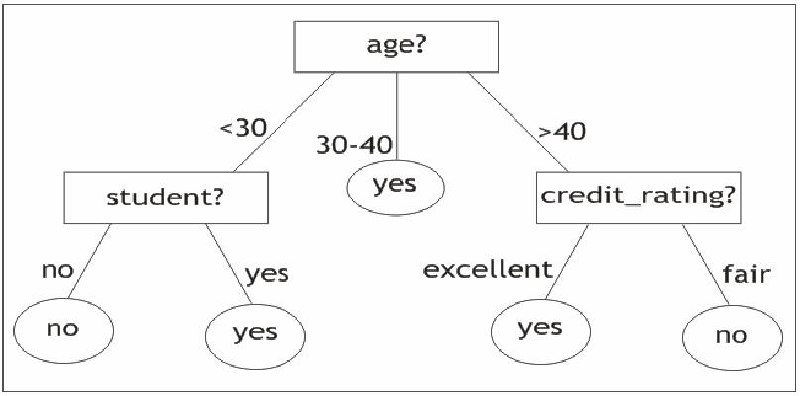
\includegraphics[width=0.85\textwidth]{images/decision-tree-buys-computer.jpg}}
    \caption{Contoh Decision Tree untuk kasus \texttt{buys\_computer} dengan atribut \texttt{age}, \texttt{student}, dan \texttt{credit\_rating}.}
    \label{fig:decision-tree}
\end{figure}

Entropi didefinisikan sebagai ukuran kemurnian split:
\begin{equation}
E(S) = -\sum_{i=1}^{m} p_i \log_2(p_i)
\end{equation}
\textit{Information Gain} untuk atribut $A$ adalah:
\begin{equation}
Gain(A) = E(S) - \sum_{j=1}^{v} \frac{|S_j|}{|S|} E(S_j)
\end{equation}
Atribut dengan \textit{gain} terbesar dipilih sebagai node pemisah. Dari pohon, aturan IF-THEN dapat diekstrak, misalnya: IF \texttt{age} = ``$<=$30'' AND \texttt{student} = ``no'' THEN \texttt{buys\_computer} = ``no''.

Untuk menghindari overfitting, dapat digunakan \textit{pre-pruning} (menghentikan konstruksi pohon lebih awal) atau \textit{post-pruning} (memangkas cabang yang tidak signifikan terhadap test set).

\subsection{Random Forest}
Random Forest adalah algoritma \textit{ensemble} yang menggabungkan banyak Decision Tree melalui teknik \textit{bagging} (\textit{bootstrap aggregating}). Setiap pohon dilatih pada subset data yang berbeda yang diambil secara \textit{sampling with replacement} (bootstrap), dan hasil akhirnya ditentukan melalui voting mayoritas. Random Forest membuat model lebih stabil, mengurangi \textit{overfitting}, dan meningkatkan akurasi dibanding satu pohon tunggal \cite{sklearn-ensemble}.

\begin{figure}[H]
    \centering
    \fbox{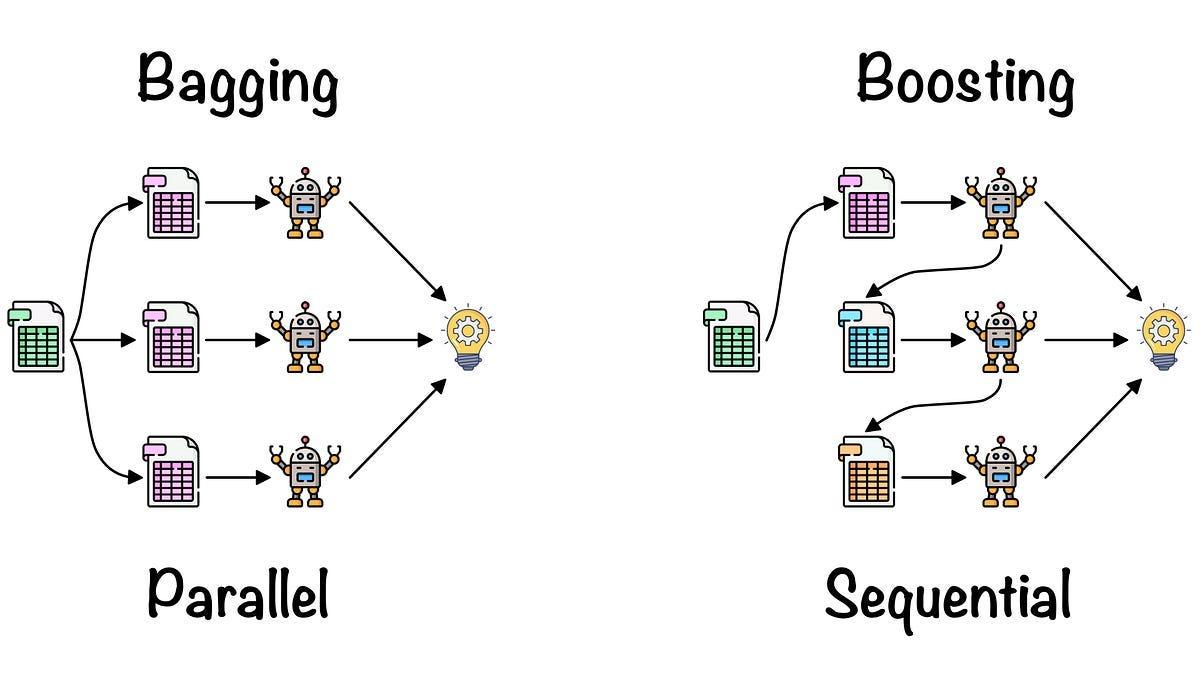
\includegraphics[width=0.9\textwidth]{images/bagging-illustration.jpg}}
    \caption{Ilustrasi Bagging: sampling with replacement untuk tiga ronde dan voting mayoritas. Contoh implementasi populer adalah Random Forest.}
    \label{fig:bagging}
\end{figure}

Analogi bagging adalah diagnosis berdasarkan suara mayoritas dari banyak dokter. Karena setiap pohon melihat variasi data yang berbeda, varians model keseluruhan berkurang tanpa meningkatkan bias secara signifikan.

\subsection{AdaBoost (Adaptive Boosting)}
AdaBoost bekerja dengan menggabungkan beberapa \textit{weak learner} (biasanya Decision Tree kecil / stump) secara berurutan. Pada setiap iterasi, bobot sampel diperbarui sehingga model berikutnya lebih fokus pada data yang sebelumnya salah diklasifikasikan. Setiap \textit{weak learner} diberi bobot berdasarkan akurasinya, dan prediksi akhir merupakan kombinasi berbobot dari seluruh learner. Dengan cara ini, AdaBoost mampu meningkatkan performa model secara signifikan terutama pada dataset yang kompleks, namun berisiko overfitting pada data yang sangat noisy \cite{sklearn-ensemble}.

\section{Metrik Evaluasi Classification}
Dalam \textit{machine learning} khususnya pada model klasifikasi, diperlukan metrik evaluasi untuk menilai seberapa baik model mampu memprediksi label dengan benar. Evaluasi ini dilakukan dengan membandingkan hasil prediksi model terhadap nilai aktual melalui sebuah struktur yang disebut \textit{confusion matrix} \cite{sklearn-metrics}.

\subsection{Confusion Matrix}
\textit{Confusion matrix} terdiri dari empat komponen penting, antara lain \textit{True Positive} (TP) yaitu prediksi positif yang benar, \textit{True Negative} (TN) yaitu prediksi negatif yang benar, \textit{False Positive} (FP) yaitu prediksi positif yang salah, dan \textit{False Negative} (FN) yaitu prediksi negatif yang salah. Berdasarkan nilai-nilai ini, beberapa metrik evaluasi dapat dihitung \cite{sklearn-metrics}.

\begin{figure}[H]
    \centering
    \fbox{
\includegraphics[width=0.7\textwidth]{images/confusion-matrix-structure.jpg}}
    \caption{Struktur Confusion Matrix 2x2 dengan komponen TP, TN, FP, dan FN.}
    \label{fig:confusion-matrix}
\end{figure}

\subsection{Accuracy, Precision, Recall, F1-Score}
\textbf{Accuracy} merupakan metrik paling dasar yang menunjukkan proporsi prediksi yang benar dari seluruh prediksi yang dibuat oleh model:
\begin{equation}
Accuracy = \frac{TP + TN}{TP + TN + FP + FN}
\end{equation}

\textbf{Precision} mengukur tingkat ketepatan model dalam melakukan prediksi positif, yaitu berapa banyak prediksi positif yang benar-benar positif:
\begin{equation}
Precision = \frac{TP}{TP + FP}
\end{equation}

\textbf{Recall} (atau \textit{sensitivity} / \textit{true positive rate}) mengukur kemampuan model dalam menemukan seluruh sampel yang benar-benar positif:
\begin{equation}
Recall = \frac{TP}{TP + FN}
\end{equation}

Karena \textit{precision} dan \textit{recall} memiliki fokus yang berbeda, \textbf{F1-Score} digunakan sebagai metrik yang menyeimbangkan keduanya. Metrik ini sangat berguna ketika dataset bersifat \textit{imbalanced} dan diperlukan keseimbangan antara kemampuan model menghindari \textit{false positives} serta \textit{false negatives}. F1-score merupakan \textit{harmonic mean} dari \textit{precision} dan \textit{recall}:
\begin{equation}
F1 = \frac{2 \times Precision \times Recall}{Precision + Recall}
\end{equation}

\textit{Accuracy} dapat menyesatkan pada dataset yang tidak seimbang. Misalnya, jika 990 dari 1000 sampel adalah kelas 0 dan model memprediksi semuanya sebagai kelas 0, akurasi mencapai 99\% namun gagal mendeteksi kelas 1 sama sekali. Oleh karena itu, \textit{precision}, \textit{recall}, dan F1 perlu diperhatikan bersamaan, terutama dengan parameter \texttt{average='macro'} agar setiap kelas memiliki kontribusi yang sama \cite{sklearn-metrics,han2022}.

\section{Validation Techniques}
Performa model dapat dipengaruhi oleh distribusi kelas, biaya kesalahan klasifikasi, serta ukuran data latih dan uji. Dua teknik validasi umum adalah:

\textbf{Holdout:} Data dibagi menjadi dua bagian, yaitu training set (misalnya 70\%) dan testing set (30\%). Model dilatih pada training set dan dievaluasi pada testing set yang tidak pernah dilihat selama pelatihan. Proporsi umum adalah 60:40, 70:30, atau 80:20 \cite{han2022}.

\textbf{Cross Validation:} Data dipartisi menjadi $k$ subset yang saling lepas. Pada $k$-fold cross validation, model dilatih pada $k-1$ partisi dan diuji pada 1 partisi yang tersisa, diulang sebanyak $k$ kali. Hasil akhir adalah rata-rata performa dari $k$ iterasi. Pada \textit{stratified} $k$-fold, setiap fold mempertahankan proporsi kelas yang sama dengan dataset asli, sehingga evaluasi lebih representatif untuk dataset yang imbalanced \cite{sklearn-cross-validation,dicoding-workflow,digitalskola-preprocessing}.

\clearpage

\chapter[\tocboldsection{Hasil dan Pembahasan}]{Hasil dan Pembahasan}

\section{Percobaan Latihan Praktikum}
Pada bagian ini saya mendokumentasikan percobaan klasifikasi sesuai langkah pada Modul Pertemuan 3. Dataset yang digunakan adalah \textit{Stroke Prediction Dataset} dari Kaggle (\url{https://www.kaggle.com/datasets/fedesoriano/stroke-prediction-dataset}) yang juga tersedia di GitHub \texttt{ganjar87/data\_science\_practice}. Setiap langkah disertai kode yang saya jalankan di Google Colaboratory beserta screenshot hasil eksekusinya. Notebook yang saya gunakan dapat diakses melalui tautan Google Colab berikut: \url{https://colab.research.google.com/drive/1u5hrJQDwnOMdlWAobI8k7-zzQ_X5HPU0?usp=sharing}.

\subsection{Persiapan dan Impor Pustaka}
Saya menyiapkan lingkungan Python dan mengimpor pustaka yang dibutuhkan untuk manipulasi data, visualisasi, dan pemodelan klasifikasi.

\begin{lstlisting}[style=pythonstyle,caption={Impor pustaka praktikum klasifikasi.}]
import pandas as pd
import numpy as np
import matplotlib.pyplot as plt
import seaborn as sns
from sklearn.model_selection import train_test_split
from sklearn.preprocessing import StandardScaler, LabelEncoder
from sklearn.impute import SimpleImputer
from sklearn.linear_model import LogisticRegression
from sklearn.neighbors import KNeighborsClassifier
from sklearn.tree import DecisionTreeClassifier
from sklearn.ensemble import RandomForestClassifier, AdaBoostClassifier
from sklearn.metrics import accuracy_score, precision_score, recall_score, f1_score, confusion_matrix, ConfusionMatrixDisplay, classification_report
\end{lstlisting}

\begin{figure}[H]
\centering
\customfbox{
\includegraphics[width=0.9\textwidth]{images/ss-01-import-library.jpg}}
\caption{Impor pustaka yang digunakan dalam praktikum klasifikasi.}
\label{fig:ss01-import}
\end{figure}

\subsection{Memuat Dataset Stroke}
Saya memuat dataset stroke yang berisi 5.110 baris dengan 12 kolom, meliputi atribut demografis, kondisi kesehatan, dan target \texttt{stroke} (0 = tidak stroke, 1 = stroke).

\begin{lstlisting}[style=pythonstyle,caption={Memuat dataset stroke.}]
df = pd.read_csv('https://raw.githubusercontent.com/ganjar87/data_science_practice/refs/heads/main/healthcare-dataset-stroke-data.csv')
df.head()
\end{lstlisting}

\begin{figure}[H]
\centering
\customfbox{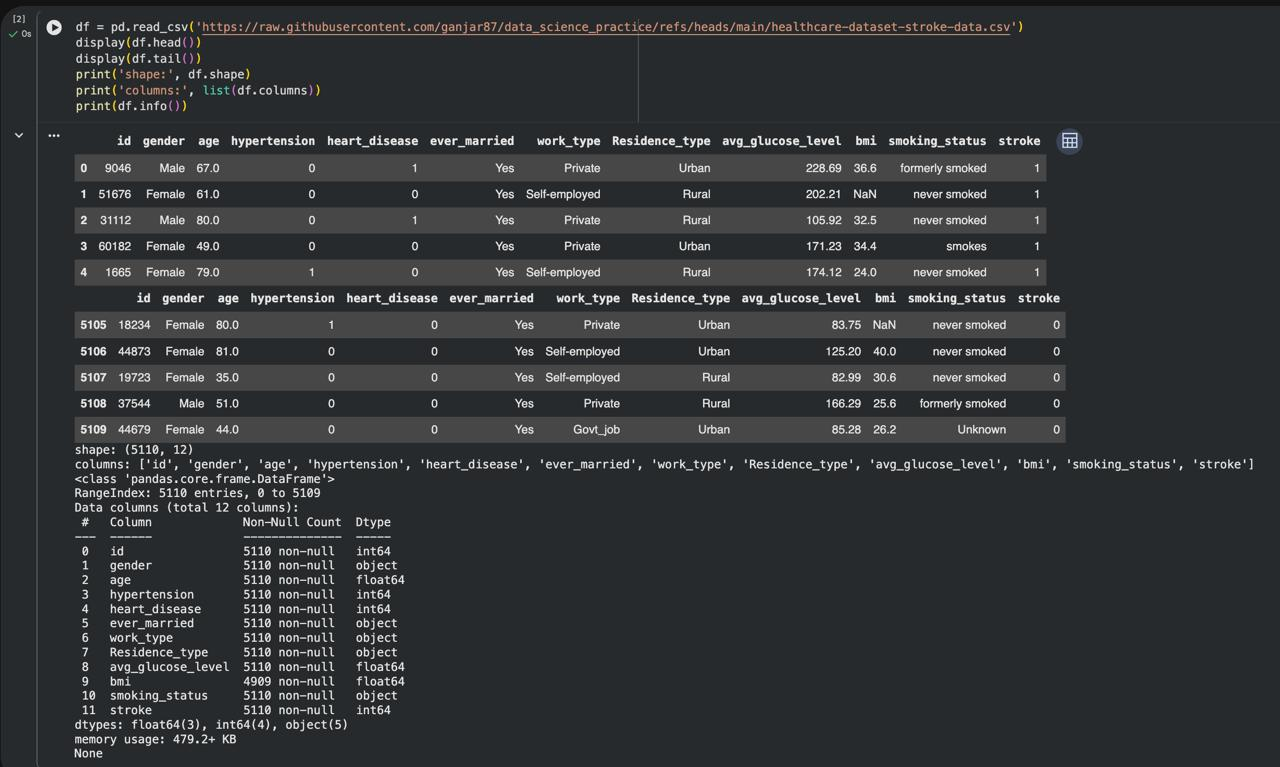
\includegraphics[width=0.9\textwidth]{images/ss-02-dataset-head.jpg}}
\caption{Lima baris pertama dataset stroke (\texttt{df.head()}).}
\label{fig:ss02-head}
\end{figure}

\begin{lstlisting}[style=pythonstyle,caption={Melihat lima baris terakhir dataset.}]
df.tail()
\end{lstlisting}

\begin{figure}[H]
\centering
\customfbox{
\includegraphics[width=0.9\textwidth]{images/ss-03-dataset-tail.jpg}}
\caption{Lima baris terakhir dataset stroke (\texttt{df.tail()}).}
\label{fig:ss03-tail}
\end{figure}

Dataset memiliki kolom \texttt{id}, \texttt{gender}, \texttt{age}, \texttt{hypertension}, \texttt{heart\_disease}, \texttt{ever\_married}, \texttt{work\_type}, \texttt{Residence\_type}, \texttt{avg\_glucose\_level}, \texttt{bmi}, \texttt{smoking\_status}, dan \texttt{stroke}.

\subsection{Exploratory Data Analysis (EDA)}

\subsubsection{Deskripsi Statistik}
Saya menggunakan \texttt{df.describe()} untuk melihat statistik deskriptif variabel numerik.

\begin{lstlisting}[style=pythonstyle,caption={Deskripsi statistik dataset.}]
df.describe()
\end{lstlisting}

\begin{figure}[H]
\centering
\customfbox{
\includegraphics[width=0.9\textwidth]{images/ss-04-describe.jpg}}
\caption{Hasil deskripsi statistik dataset (\texttt{df.describe()}). Terlihat count untuk \texttt{bmi} hanya 4.909 dari 5.110, mengindikasikan 201 missing value.}
\label{fig:ss04-describe}
\end{figure}

Rata-rata usia (\texttt{age}) adalah 43,22 tahun, rata-rata \texttt{avg\_glucose\_level} 106,15, dan rata-rata \texttt{stroke} 0,048 (4,8\%), yang sudah mengindikasikan ketidakseimbangan kelas.

\subsubsection{Presentase Target Kelas}
Saya memvisualisasikan distribusi target menggunakan pie chart.

\begin{lstlisting}[style=pythonstyle,caption={Presentase target kelas.}]
data = df['stroke'].value_counts()
data.plot(kind='pie', autopct='%.2f%%')
plt.title('Distribusi Kelas Stroke')
plt.ylabel('')
plt.show()
\end{lstlisting}

\begin{figure}[H]
\centering
\customfbox{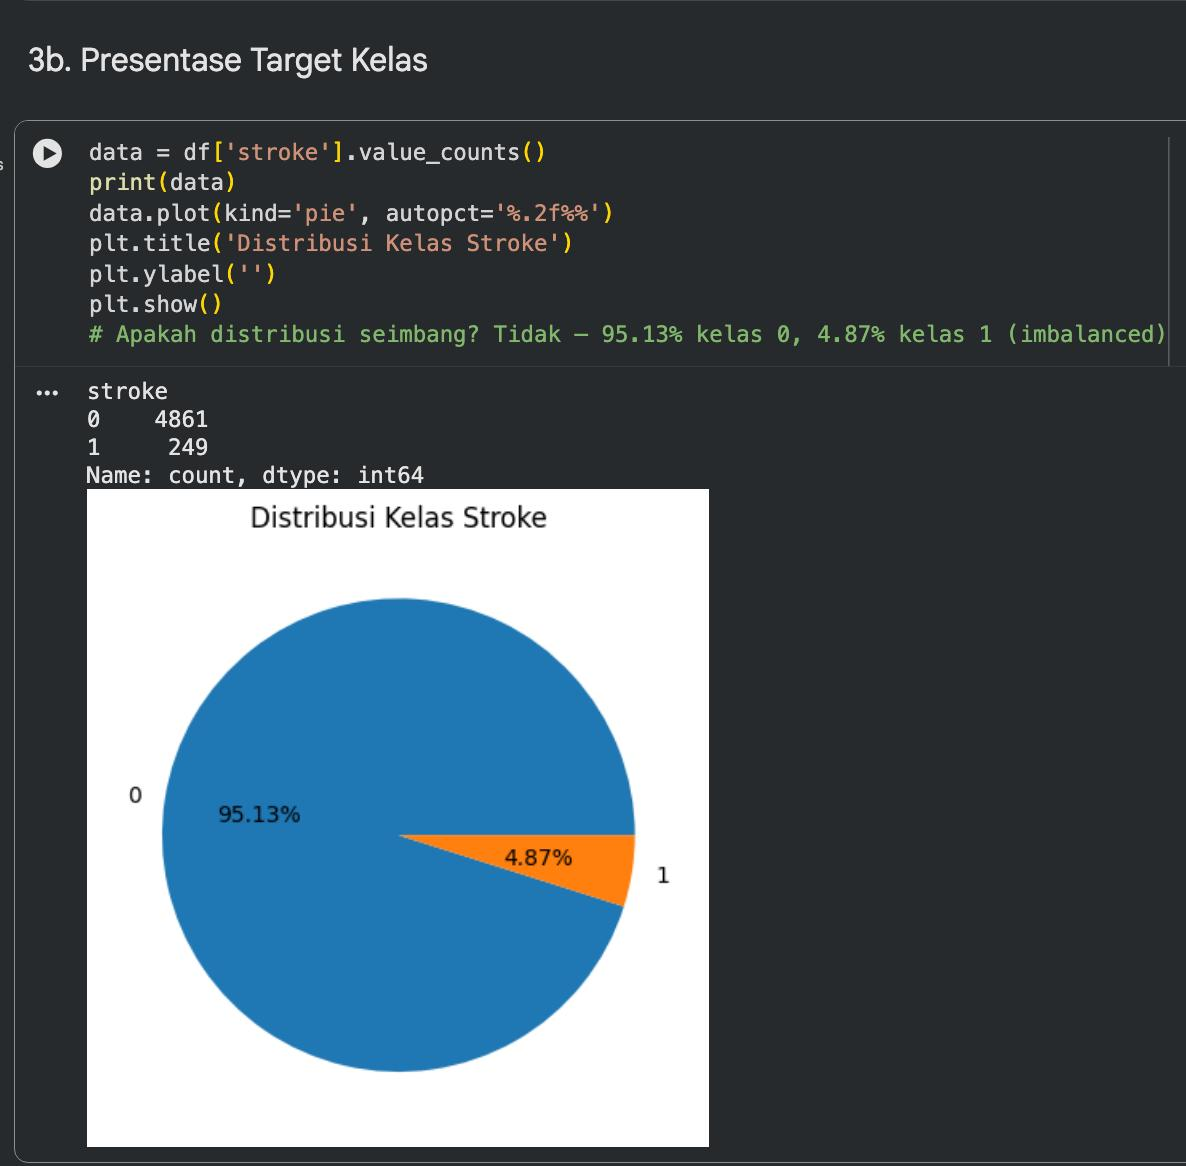
\includegraphics[width=0.6\textwidth]{images/ss-05-pie-target.jpg}}
\caption{Pie chart distribusi variabel target \texttt{stroke}: kelas 0 (tidak stroke) 95,13\% dan kelas 1 (stroke) 4,87\% — dataset bersifat imbalanced.}
\label{fig:ss05-pie}
\end{figure}

\subsubsection{Histogram Variabel Numerik}
Saya membuat histogram untuk melihat distribusi dan skewness variabel numerik.

\begin{lstlisting}[style=pythonstyle,caption={Kode untuk menampilkan histogram.}]
df.hist(figsize=(10,10))
plt.tight_layout()
plt.show()
\end{lstlisting}

\begin{figure}[H]
\centering
\customfbox{
\includegraphics[width=0.7\textwidth]{images/ss-06-histogram-code.jpg}}
\caption{Kode untuk menampilkan histogram seluruh variabel numerik.}
\label{fig:ss06-hist-code}
\end{figure}

\begin{figure}[H]
\centering
\customfbox{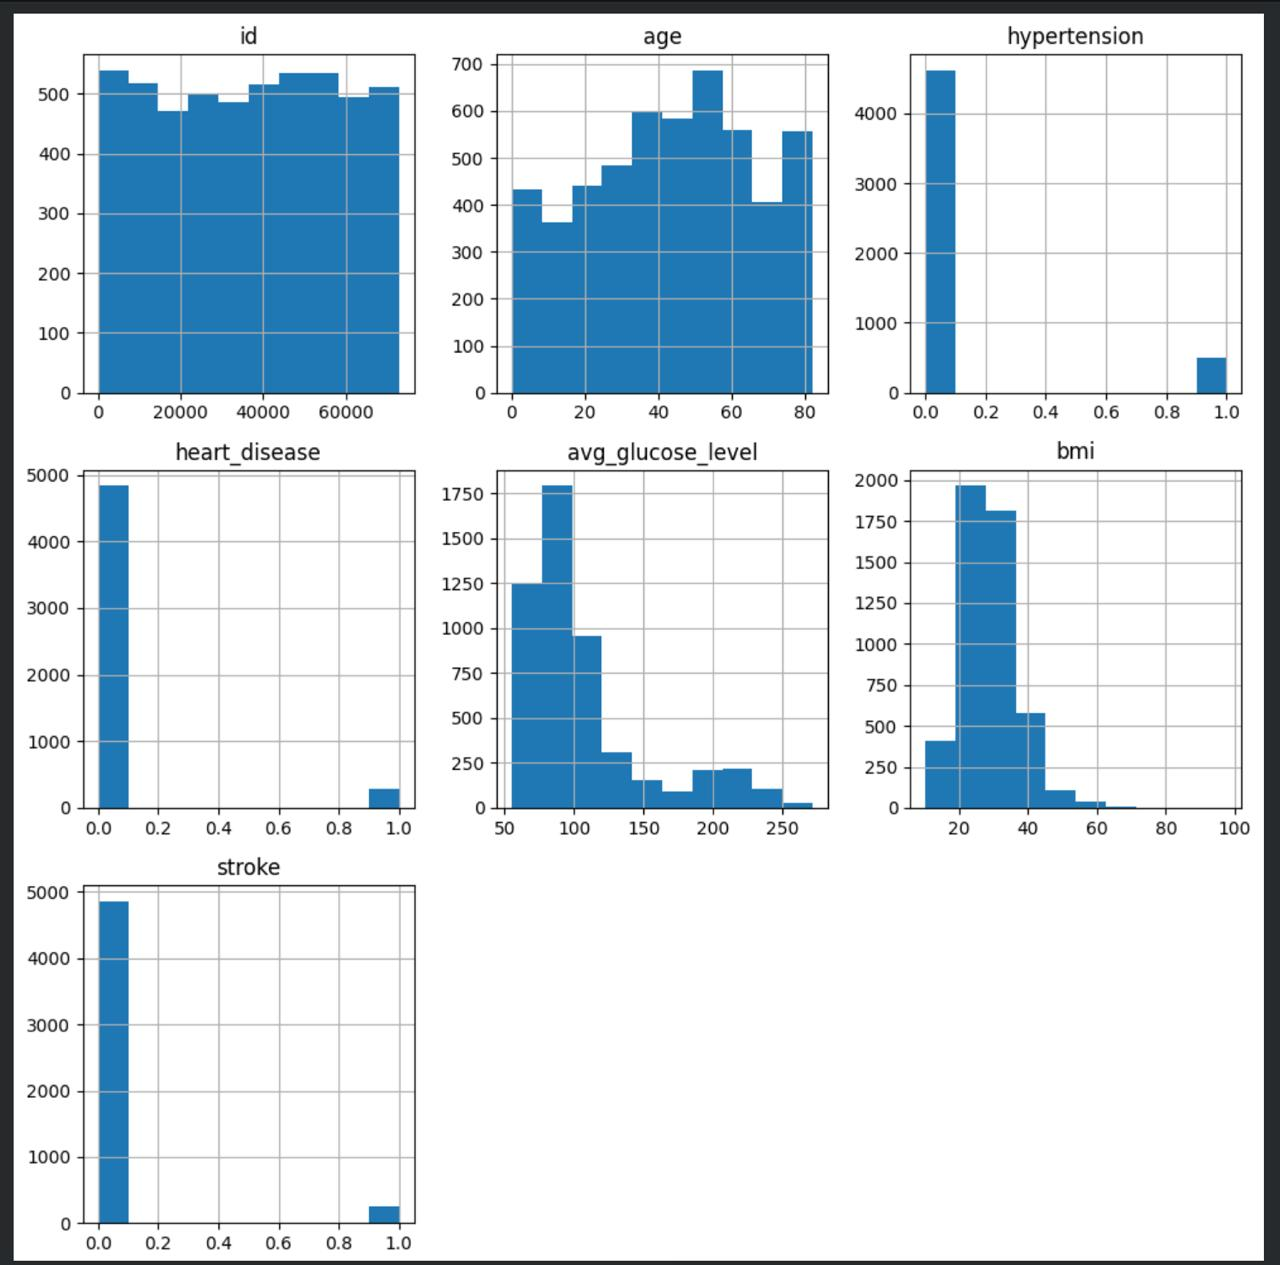
\includegraphics[width=0.9\textwidth]{images/ss-07-histogram-result.jpg}}
\caption{Histogram seluruh variabel numerik. Variabel \texttt{age} agak normal dengan sedikit skew ke kanan, sedangkan \texttt{avg\_glucose\_level} dan \texttt{bmi} right-skewed mengindikasikan outlier.}
\label{fig:ss07-hist-result}
\end{figure}

\subsubsection{Pengecekan Missing Value}
Saya memeriksa jumlah missing value pada setiap kolom.

\begin{lstlisting}[style=pythonstyle,caption={Pengecekan missing value.}]
df.isnull().sum()
\end{lstlisting}

\begin{figure}[H]
\centering
\customfbox{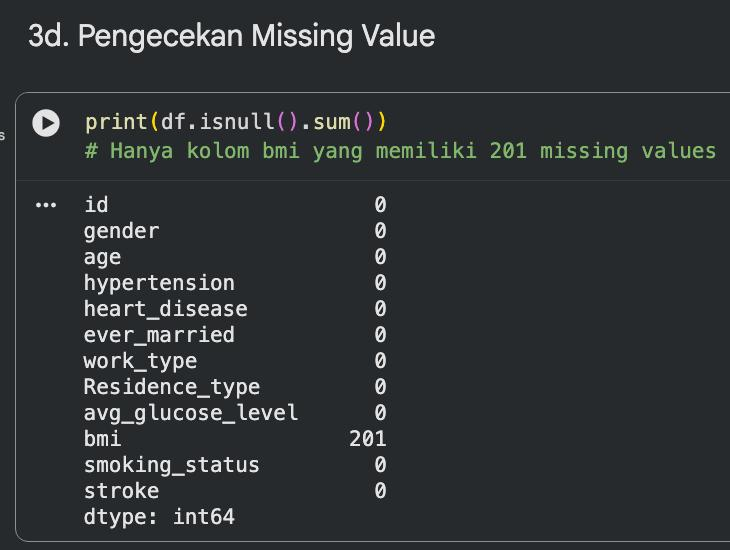
\includegraphics[width=0.7\textwidth]{images/ss-08-missing-value.jpg}}
\caption{Hasil pengecekan missing value: hanya kolom \texttt{bmi} yang memiliki 201 missing value, kolom lain 0.}
\label{fig:ss08-missing}
\end{figure}

\subsubsection{Pengecekan Atribut Kategorikal}
Saya mengidentifikasi kolom kategorikal yang memerlukan encoding.

\begin{lstlisting}[style=pythonstyle,caption={Pengecekan atribut kategorikal.}]
df_X = df.drop(['id', 'stroke'], axis=1)
cats = df_X.select_dtypes(include=['object', 'bool']).columns
print(cats.tolist())
\end{lstlisting}

\begin{figure}[H]
\centering
\customfbox{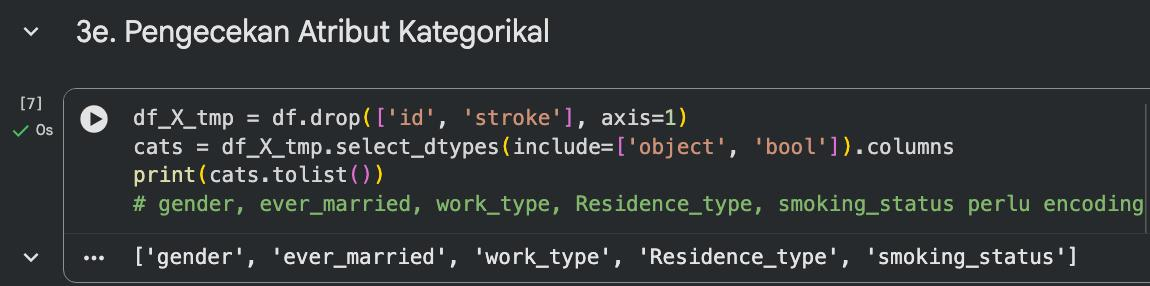
\includegraphics[width=0.7\textwidth]{images/ss-09-categorical.jpg}}
\caption{Hasil pengecekan atribut kategorikal: \texttt{gender}, \texttt{ever\_married}, \texttt{work\_type}, \texttt{Residence\_type}, dan \texttt{smoking\_status}.}
\label{fig:ss09-categorical}
\end{figure}

Kolom-kolom tersebut perlu diubah menjadi numerik sebelum pemodelan.

\subsection{Data Preprocessing}
Tahap preprocessing meliputi pemisahan fitur dan target, imputasi, encoding, konversi ke array, pembagian data, dan scaling. Saya menggunakan \texttt{SimpleImputer(strategy='median')} untuk kolom \texttt{bmi}, \texttt{LabelEncoder} untuk kolom kategorikal, \texttt{train\_test\_split} dengan proporsi 70:30, dan \texttt{StandardScaler} yang di-fit hanya pada data latih.

\begin{lstlisting}[style=pythonstyle,caption={Kode data preprocessing lengkap.}]
from sklearn.model_selection import train_test_split
from sklearn.preprocessing import LabelEncoder, StandardScaler

# Pemisahan fitur dan target
df_X = df.drop(['id', 'stroke'], axis=1)
df_y = df[['stroke']]

# Label encoding untuk target
le = LabelEncoder()
df_y = le.fit_transform(df_y['stroke'])

# Imputasi nilai hilang pada bmi dengan median
df_X['bmi'].fillna(df_X['bmi'].median(), inplace=True)

# Categorical encoding untuk kolom objek
cats = df_X.select_dtypes(include=['object', 'bool']).columns
cat_features = list(cats.values)
le = LabelEncoder()
for i in cat_features:
    df_X[i] = le.fit_transform(df_X[i])

# Konversi ke numpy array float
X = df_X.astype(float).values
y = df_y.astype(float)

# Hold-out split 70:30
X_train, X_test, y_train, y_test = train_test_split(X, y, test_size=0.3, random_state=42)

# Scaling (fit hanya pada X_train)
scaler = StandardScaler().fit(X_train)
X_train = scaler.transform(X_train)
X_test = scaler.transform(X_test)
\end{lstlisting}

\begin{figure}[H]
\centering
\customfbox{
\includegraphics[width=0.9\textwidth]{images/ss-10-preprocessing-code.jpg}}
\caption{Blok kode preprocessing: pemisahan X/y, imputasi median, encoding kategorikal, konversi array, split 70:30, dan StandardScaler.}
\label{fig:ss10-preprocessing}
\end{figure}

\textbf{Pemeriksaan hasil preprocessing:}

\begin{lstlisting}[style=pythonstyle,caption={Pemeriksaan variabel X dan y setelah preprocessing.}]
print(X[:5])
print(y[:10])
print(X_train[:3])
print(X_test[:3])
\end{lstlisting}

\begin{figure}[H]
\centering
\customfbox{
\includegraphics[width=0.9\textwidth]{images/ss-11-X-numeric.jpg}}
\caption{Variabel input X setelah dikonversi menjadi numerik (seluruh kategori telah menjadi angka).}
\label{fig:ss11-X}
\end{figure}

\begin{figure}[H]
\centering
\customfbox{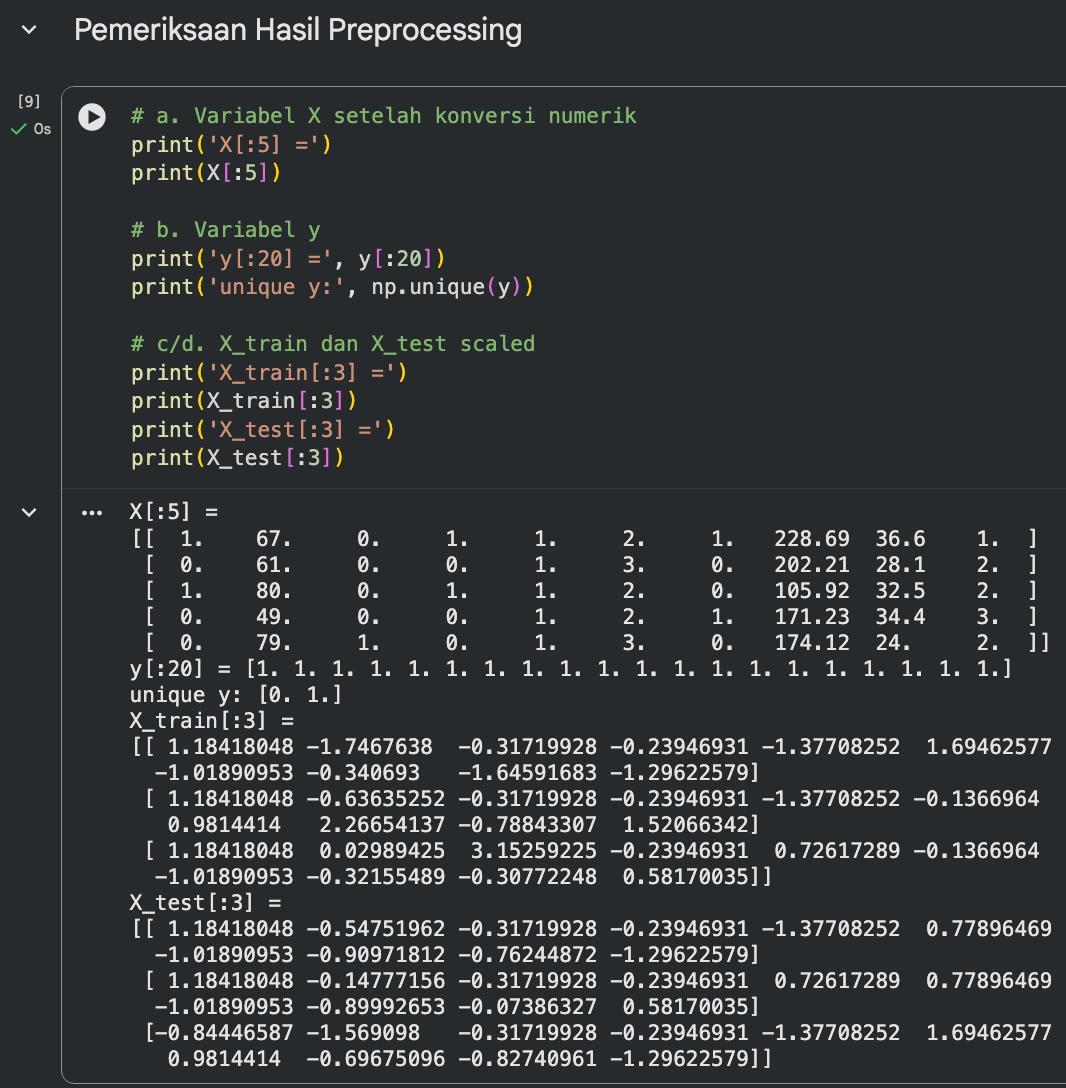
\includegraphics[width=0.6\textwidth]{images/ss-12-y-encoded.jpg}}
\caption{Variabel target y setelah label encoding (hanya berisi 0 dan 1).}
\label{fig:ss12-y}
\end{figure}

\begin{figure}[H]
\centering
\customfbox{
\includegraphics[width=0.9\textwidth]{images/ss-13-X-train-scaled.jpg}}
\caption{Hasil transformasi pada data training (X\_train) — nilai terstandarisasi dengan rata-rata sekitar 0.}
\label{fig:ss13-xtrain}
\end{figure}

\begin{figure}[H]
\centering
\customfbox{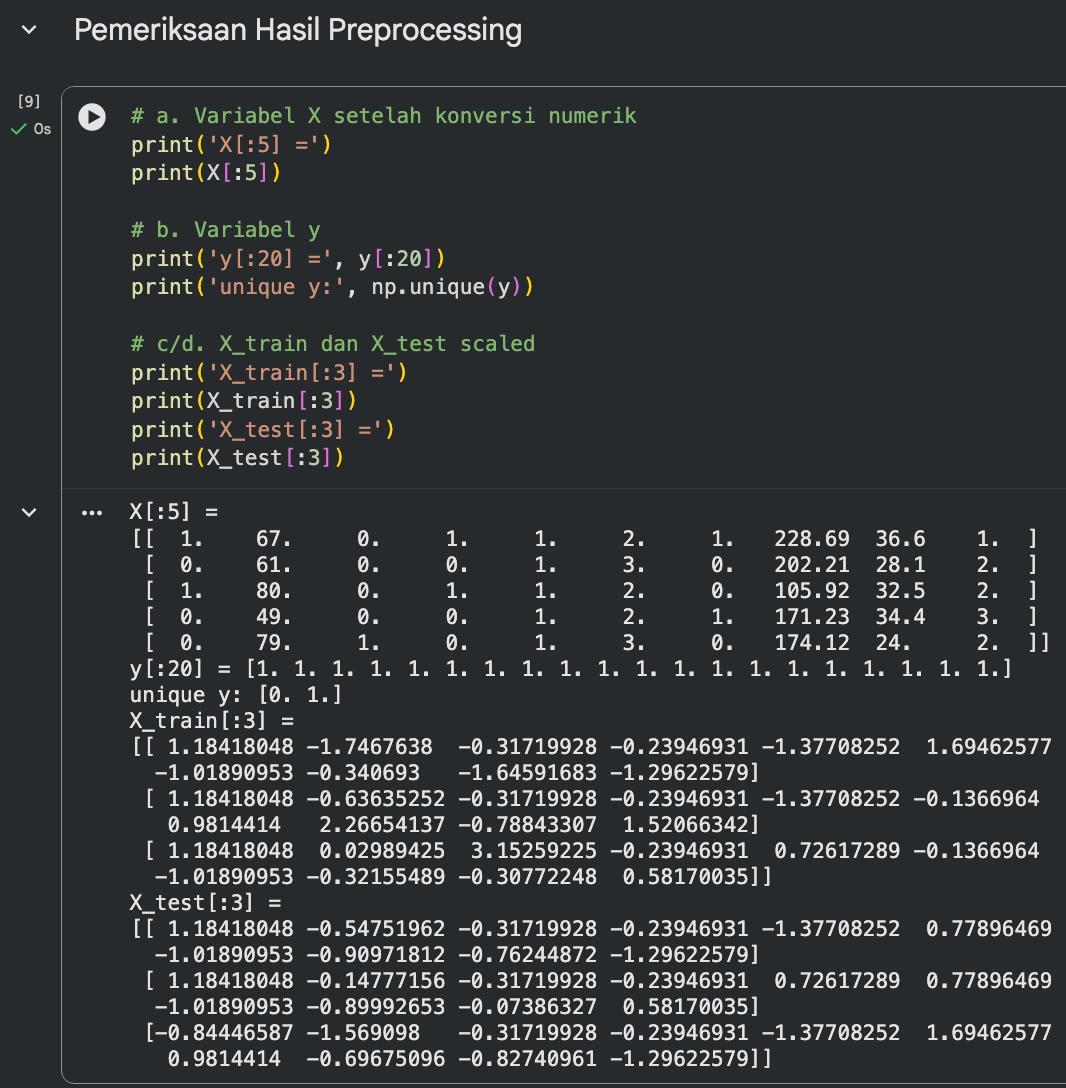
\includegraphics[width=0.9\textwidth]{images/ss-14-X-test-scaled.jpg}}
\caption{Hasil transformasi pada data testing (X\_test) — skala konsisten dengan X\_train tanpa data leakage.}
\label{fig:ss14-xtest}
\end{figure}

\subsection{Modelling}

\subsubsection{a. Logistic Regression}
Saya melatih model Logistic Regression dengan parameter default, membuat prediksi, dan mengukur performa menggunakan accuracy, precision, recall, confusion matrix, serta F1-score. Parameter \texttt{average='macro'} digunakan agar setiap kelas memiliki bobot yang sama mengingat dataset imbalanced.

\begin{lstlisting}[style=pythonstyle,caption={Kode Logistic Regression.}]
from sklearn.linear_model import LogisticRegression
from sklearn.metrics import accuracy_score, precision_score, recall_score, confusion_matrix, ConfusionMatrixDisplay, f1_score
import numpy as np

model = LogisticRegression()
model.fit(X_train, y_train)
y_pred = model.predict(X_test)

print('Accuracy ', accuracy_score(y_test, y_pred))
print('Precision ', precision_score(y_test, y_pred, average='macro'))
print('Recall ', recall_score(y_test, y_pred, average='macro'))
print('Confusion matrix ', confusion_matrix(y_test, y_pred))
cm = confusion_matrix(y_test, y_pred)
disp = ConfusionMatrixDisplay(confusion_matrix=cm, display_labels=np.unique(y_test))
disp.plot(cmap=plt.cm.Blues)
plt.show()
print('F1 ', f1_score(y_test, y_pred, average='macro'))
print(model.coef_)
print(model.intercept_)
\end{lstlisting}

\begin{figure}[H]
\centering
\customfbox{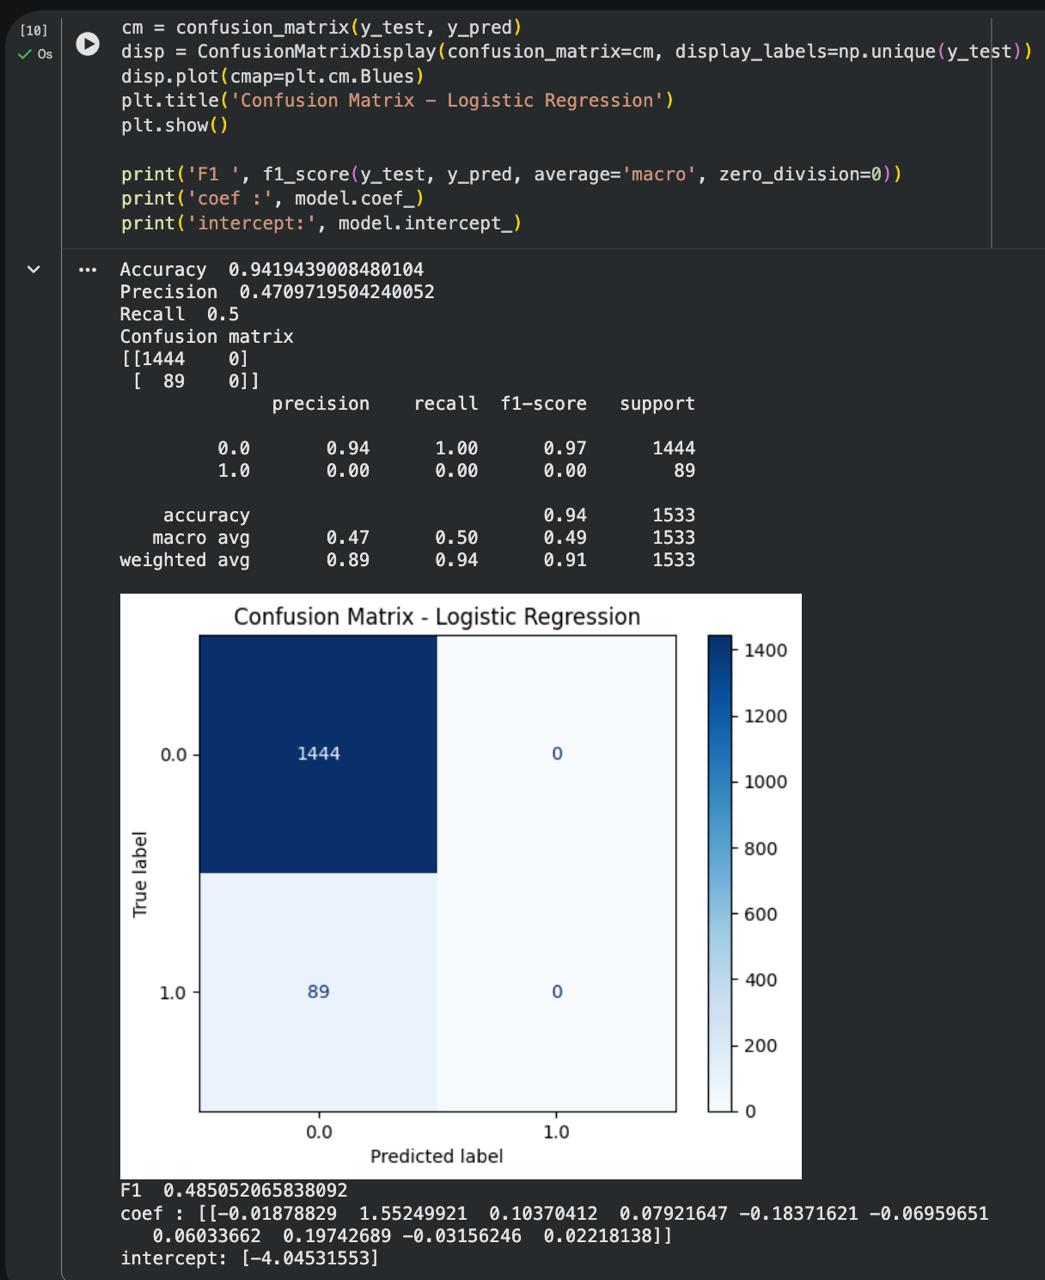
\includegraphics[width=0.9\textwidth]{images/ss-15-logreg-code.jpg}}
\caption{Kode inisialisasi, fit, dan prediksi Logistic Regression.}
\label{fig:ss15-logreg-code}
\end{figure}

\begin{figure}[H]
\centering
\customfbox{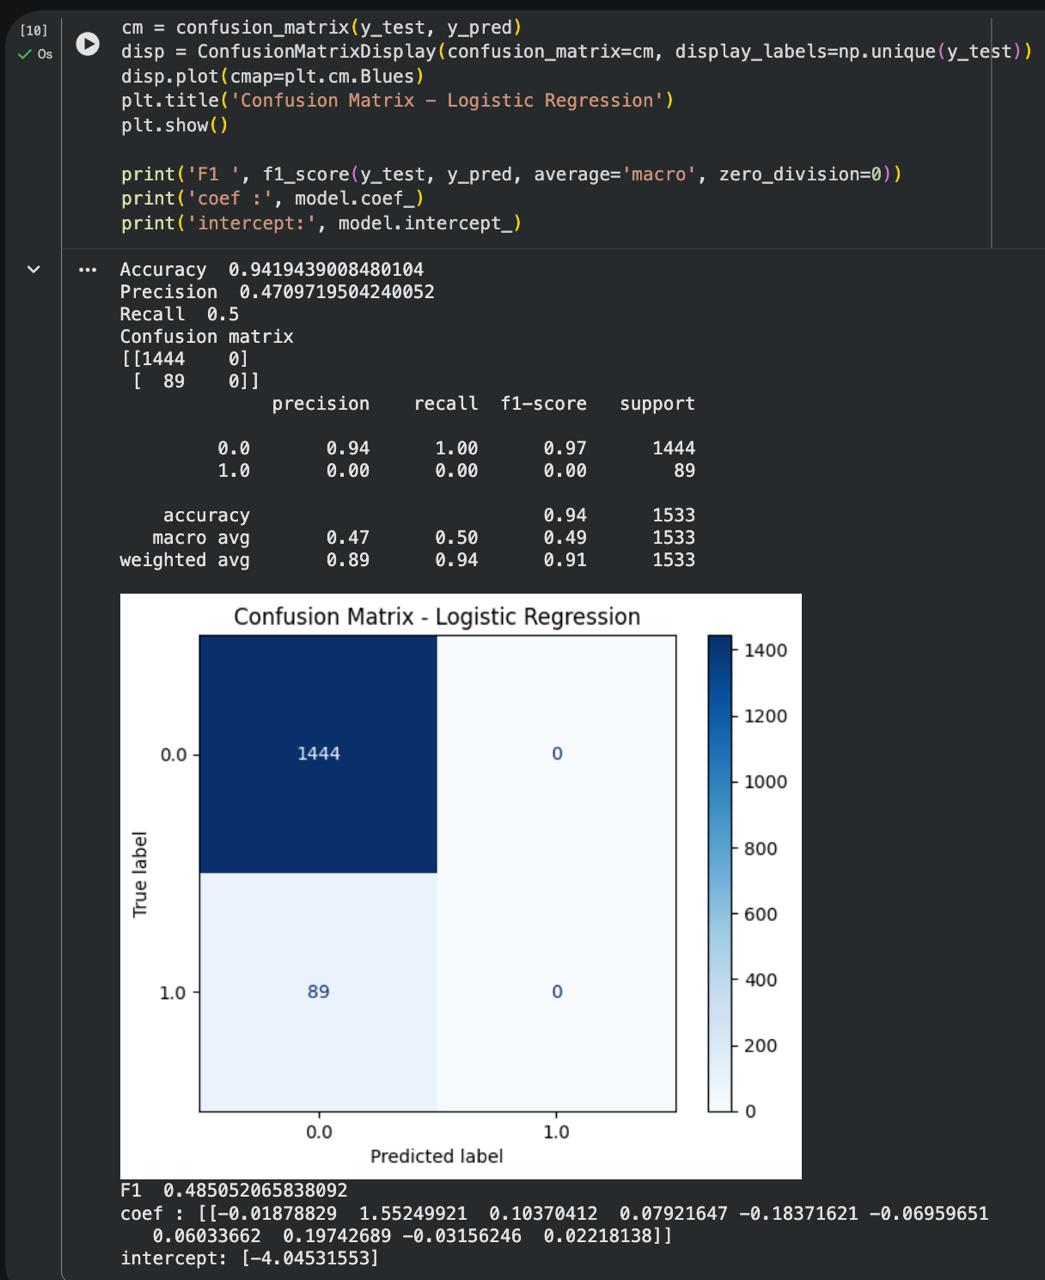
\includegraphics[width=0.9\textwidth]{images/ss-16-logreg-performance.jpg}}
\caption{Output performa Logistic Regression: Accuracy 0.9419, Precision 0.4709, Recall 0.5000, Confusion Matrix [[1444, 0], [89, 0]], F1 0.4850. Model memprediksi semua sebagai kelas 0 sehingga precision untuk kelas 1 menjadi 0.}
\label{fig:ss16-logreg-perf}
\end{figure}

\begin{figure}[H]
\centering
\customfbox{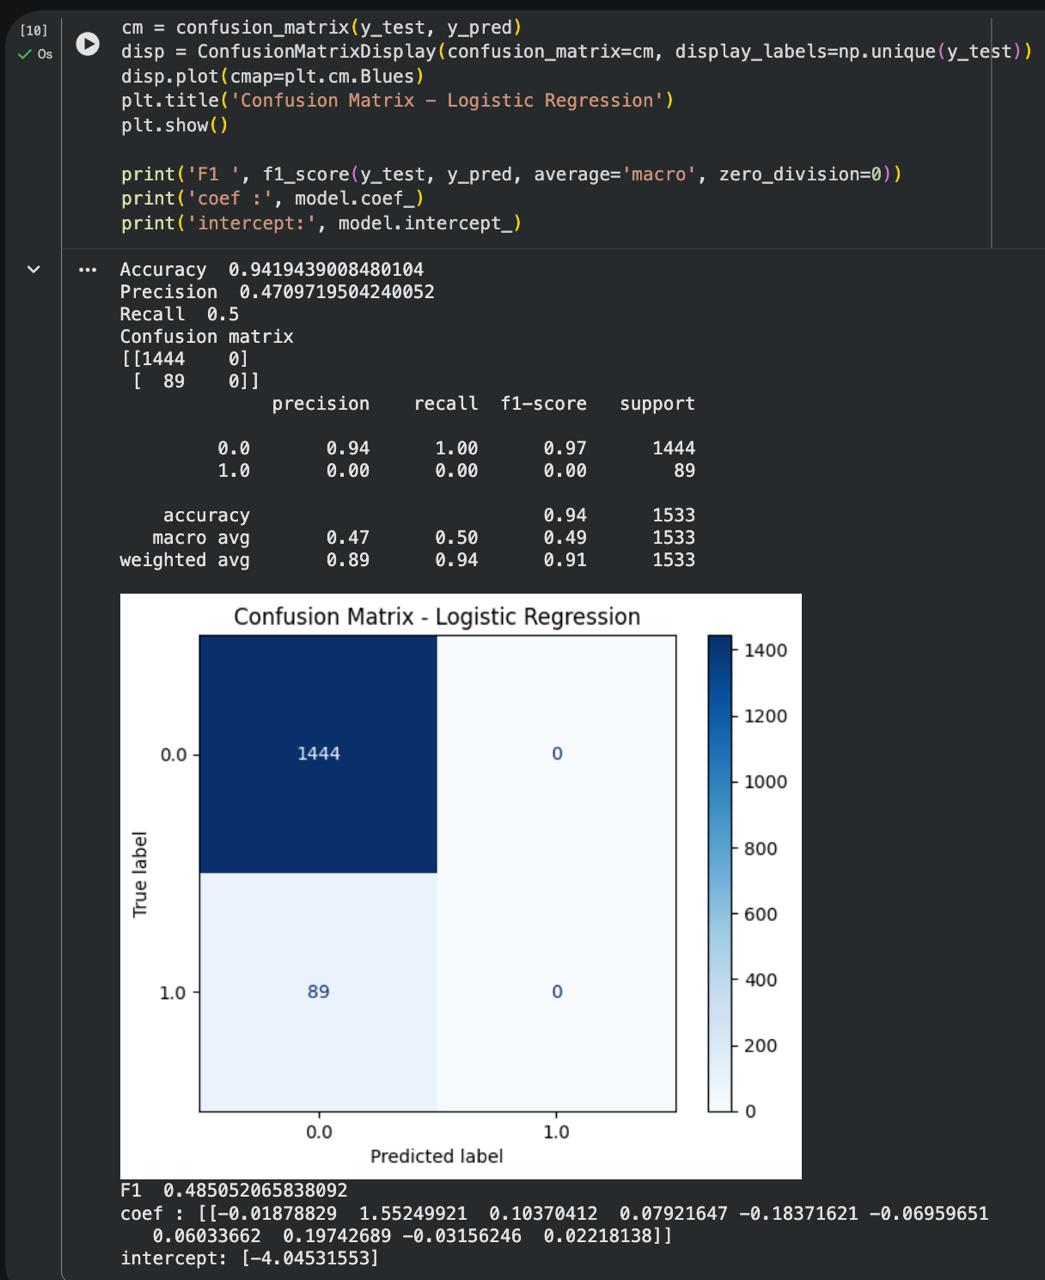
\includegraphics[width=0.6\textwidth]{images/ss-17-logreg-cm.jpg}}
\caption{Visualisasi Confusion Matrix Logistic Regression (heatmap biru: 1444 TN, 89 FN, 0 FP/TP).}
\label{fig:ss17-logreg-cm}
\end{figure}

\begin{figure}[H]
\centering
\customfbox{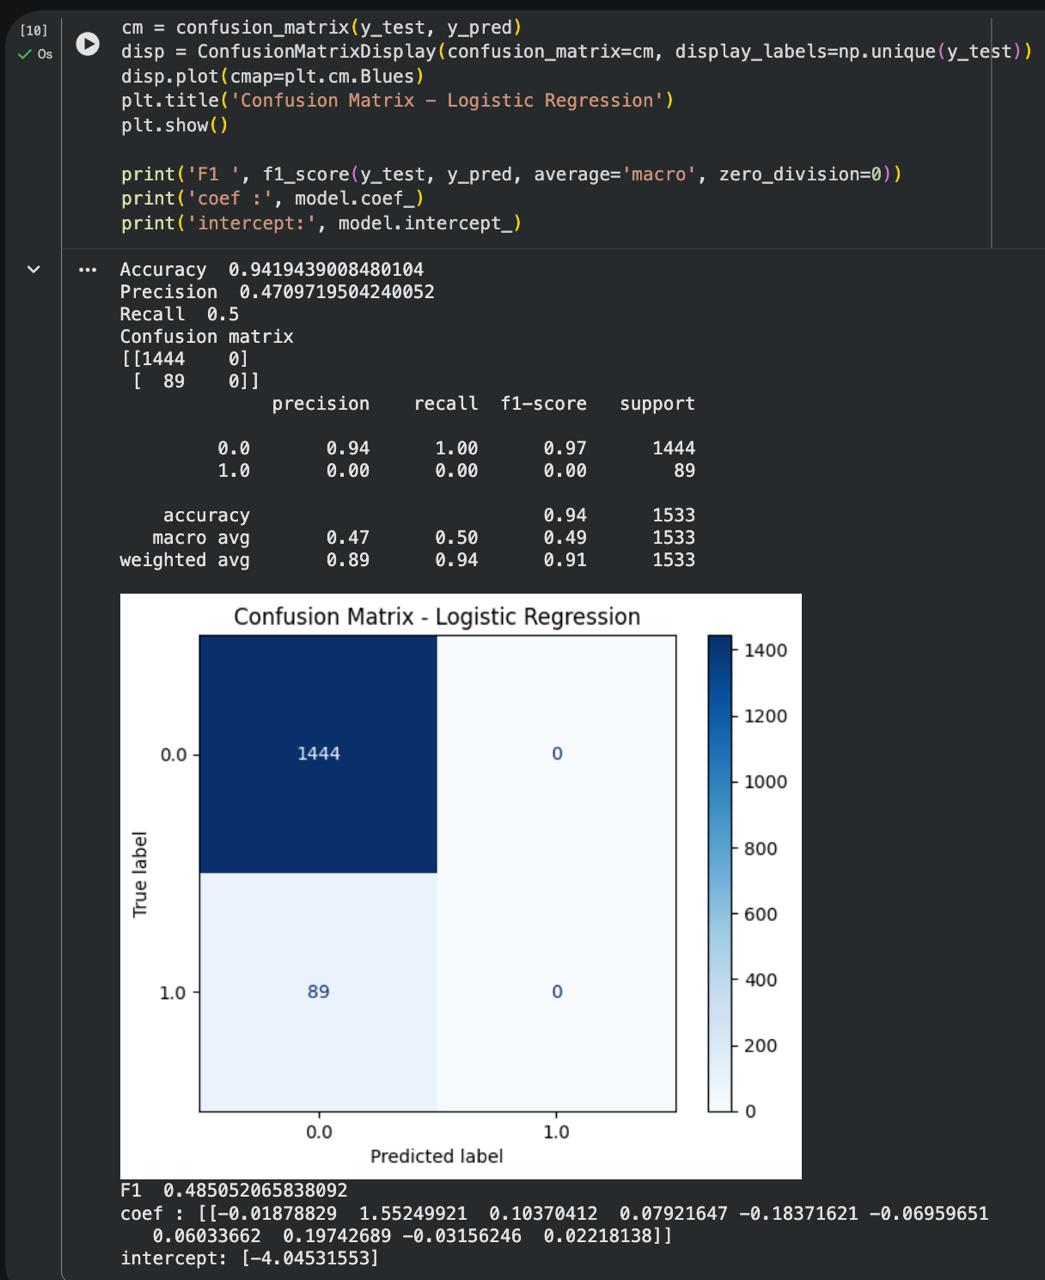
\includegraphics[width=0.6\textwidth]{images/ss-18-logreg-f1.jpg}}
\caption{Output F1-Score Logistic Regression (0.4850).}
\label{fig:ss18-logreg-f1}
\end{figure}

Saya juga memeriksa koefisien dan intercept model:

\begin{figure}[H]
\centering
\customfbox{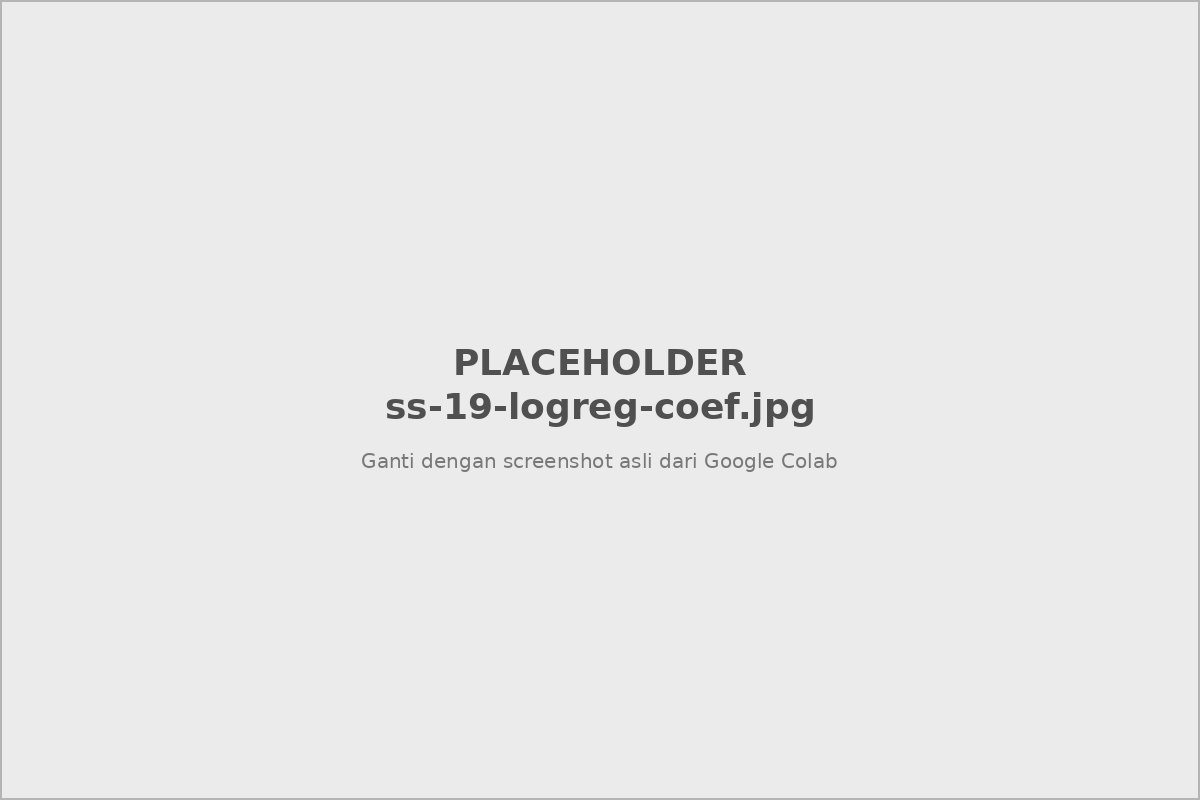
\includegraphics[width=0.9\textwidth]{images/ss-19-logreg-coef.jpg}}
\caption{Nilai koefisien Logistic Regression (\texttt{model.coef\_}): array 10 fitur dengan bobot terbesar pada fitur age (1.55).}
\label{fig:ss19-logreg-coef}
\end{figure}

\begin{figure}[H]
\centering
\customfbox{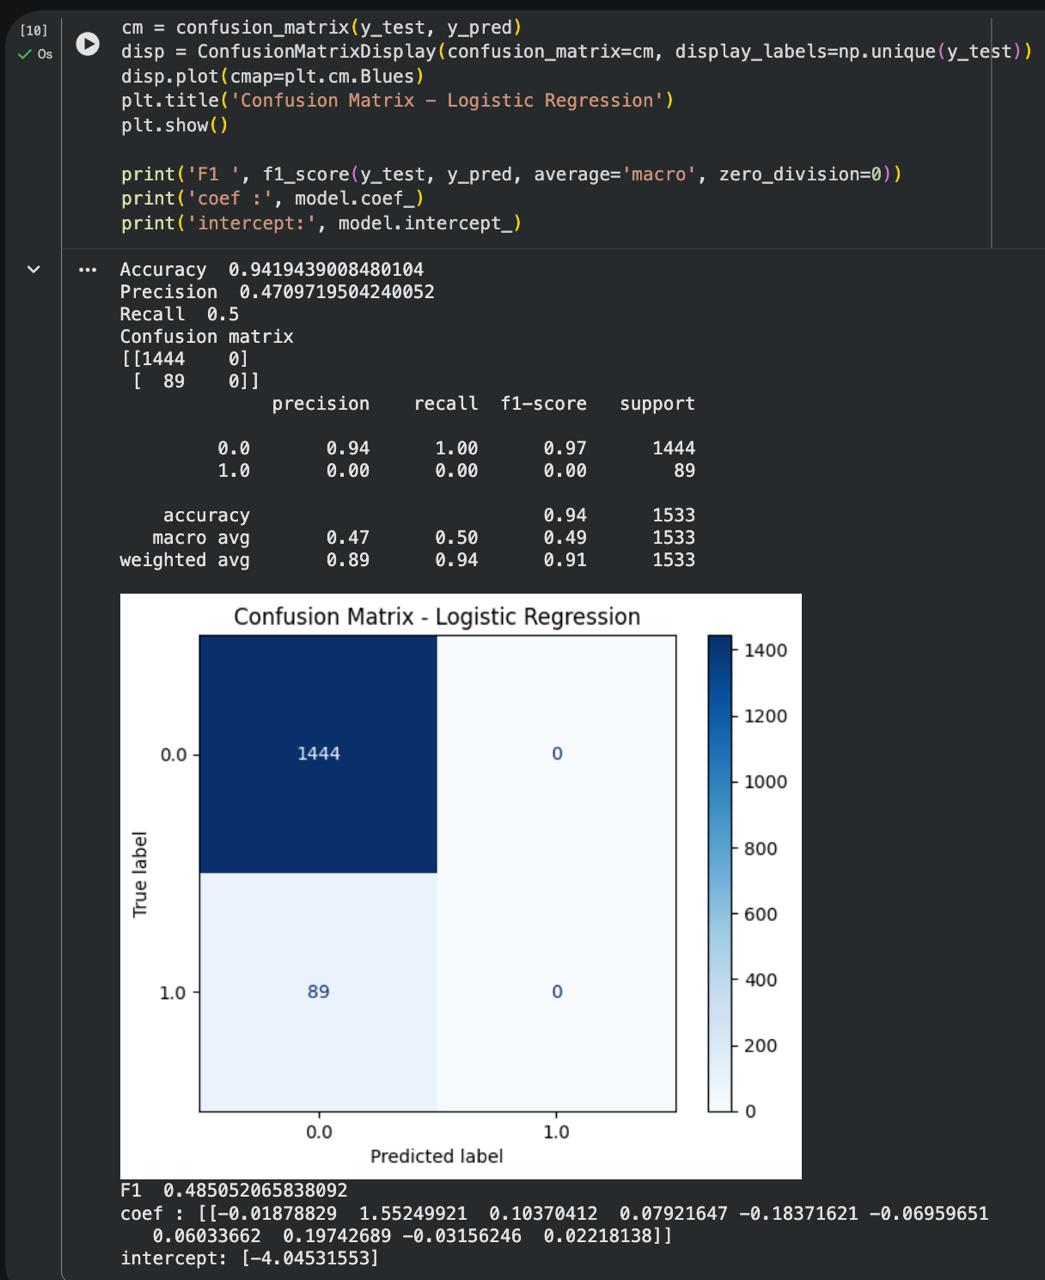
\includegraphics[width=0.6\textwidth]{images/ss-20-logreg-intercept.jpg}}
\caption{Nilai intercept Logistic Regression (\texttt{model.intercept\_}): -4.04 (bias awal negatif).}
\label{fig:ss20-logreg-intercept}
\end{figure}

\subsubsection{b. K-Nearest Neighbors (KNN)}
Saya melatih KNN dengan $k=10$ sesuai modul.

\begin{lstlisting}[style=pythonstyle,caption={Kode KNN dengan k=10.}]
from sklearn.neighbors import KNeighborsClassifier
model = KNeighborsClassifier(n_neighbors=10)
model.fit(X_train, y_train)
y_pred = model.predict(X_test)
print('Accuracy ', accuracy_score(y_test, y_pred))
print('Precision ', precision_score(y_test, y_pred, average='macro'))
print('Recall ', recall_score(y_test, y_pred, average='macro'))
print('Confusion matrix ', confusion_matrix(y_test, y_pred))
cm = confusion_matrix(y_test, y_pred)
disp = ConfusionMatrixDisplay(confusion_matrix=cm, display_labels=np.unique(y_test))
disp.plot(cmap=plt.cm.Blues)
plt.show()
\end{lstlisting}

\begin{figure}[H]
\centering
\customfbox{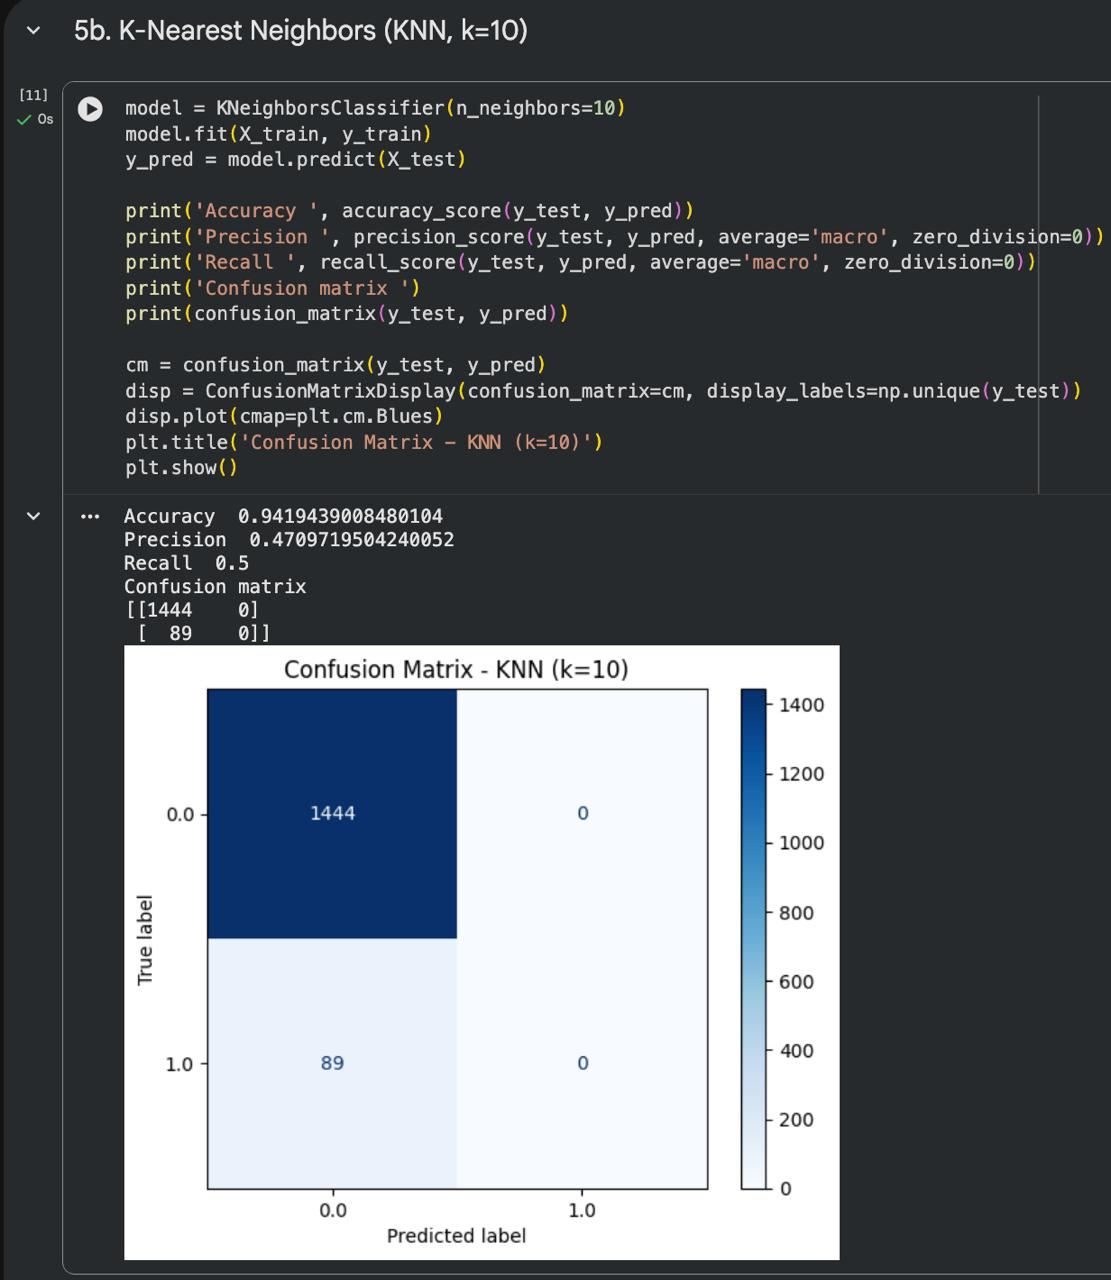
\includegraphics[width=0.9\textwidth]{images/ss-21-knn-code.jpg}}
\caption{Kode pelatihan KNN ($k=10$) dan prediksi.}
\label{fig:ss21-knn-code}
\end{figure}

\begin{figure}[H]
\centering
\customfbox{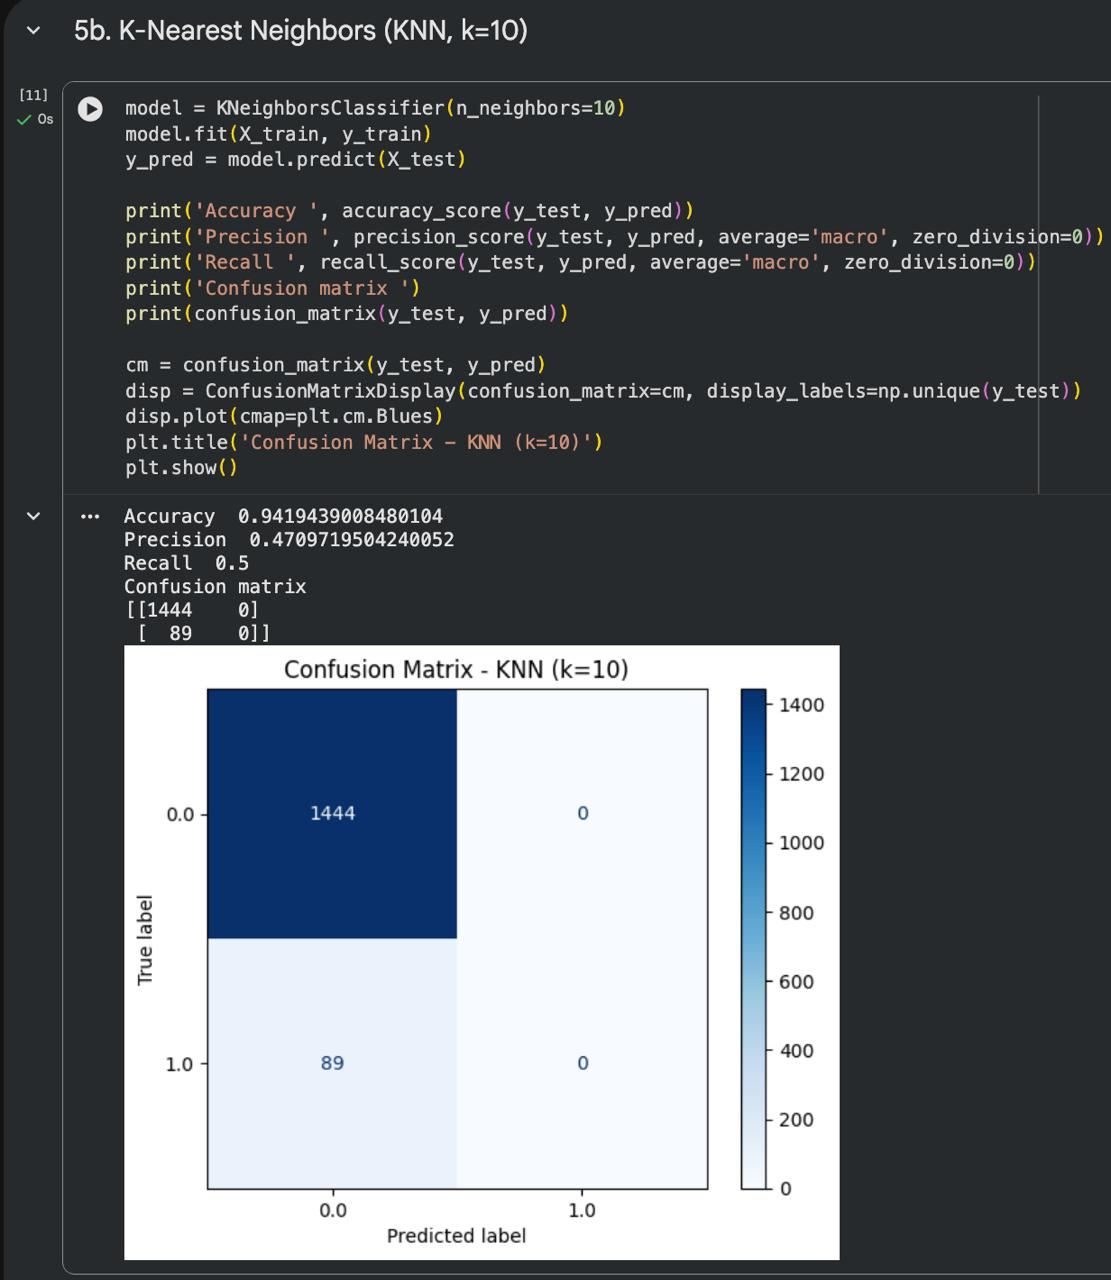
\includegraphics[width=0.9\textwidth]{images/ss-22-knn-performance.jpg}}
\caption{Output performa KNN: Accuracy 0.9419, Precision 0.4709, Recall 0.5000, Confusion Matrix [[1444, 0], [89, 0]] — identik dengan Logistic Regression, gagal mendeteksi kelas minoritas.}
\label{fig:ss22-knn-perf}
\end{figure}

\begin{figure}[H]
\centering
\customfbox{
\includegraphics[width=0.6\textwidth]{images/ss-23-knn-cm.jpg}}
\caption{Confusion Matrix KNN — 1444 True Negative dan 89 False Negative tanpa True Positive.}
\label{fig:ss23-knn-cm}
\end{figure}

\subsubsection{c. Decision Tree}
Saya melatih Decision Tree dengan kriteria \texttt{entropy}.

\begin{lstlisting}[style=pythonstyle,caption={Kode Decision Tree.}]
from sklearn.tree import DecisionTreeClassifier
model = DecisionTreeClassifier(criterion="entropy", random_state=42)
model.fit(X_train, y_train)
y_pred = model.predict(X_test)
print('Accuracy ', accuracy_score(y_test, y_pred))
print('Precision ', precision_score(y_test, y_pred, average='macro'))
print('Recall ', recall_score(y_test, y_pred, average='macro'))
print('Confusion matrix ', confusion_matrix(y_test, y_pred))
cm = confusion_matrix(y_test, y_pred)
disp = ConfusionMatrixDisplay(confusion_matrix=cm, display_labels=np.unique(y_test))
disp.plot(cmap=plt.cm.Blues)
plt.show()
\end{lstlisting}

\begin{figure}[H]
\centering
\customfbox{
\includegraphics[width=0.9\textwidth]{images/ss-24-dt-code.jpg}}
\caption{Kode pelatihan Decision Tree dengan \texttt{criterion='entropy'}.}
\label{fig:ss24-dt-code}
\end{figure}

\begin{figure}[H]
\centering
\customfbox{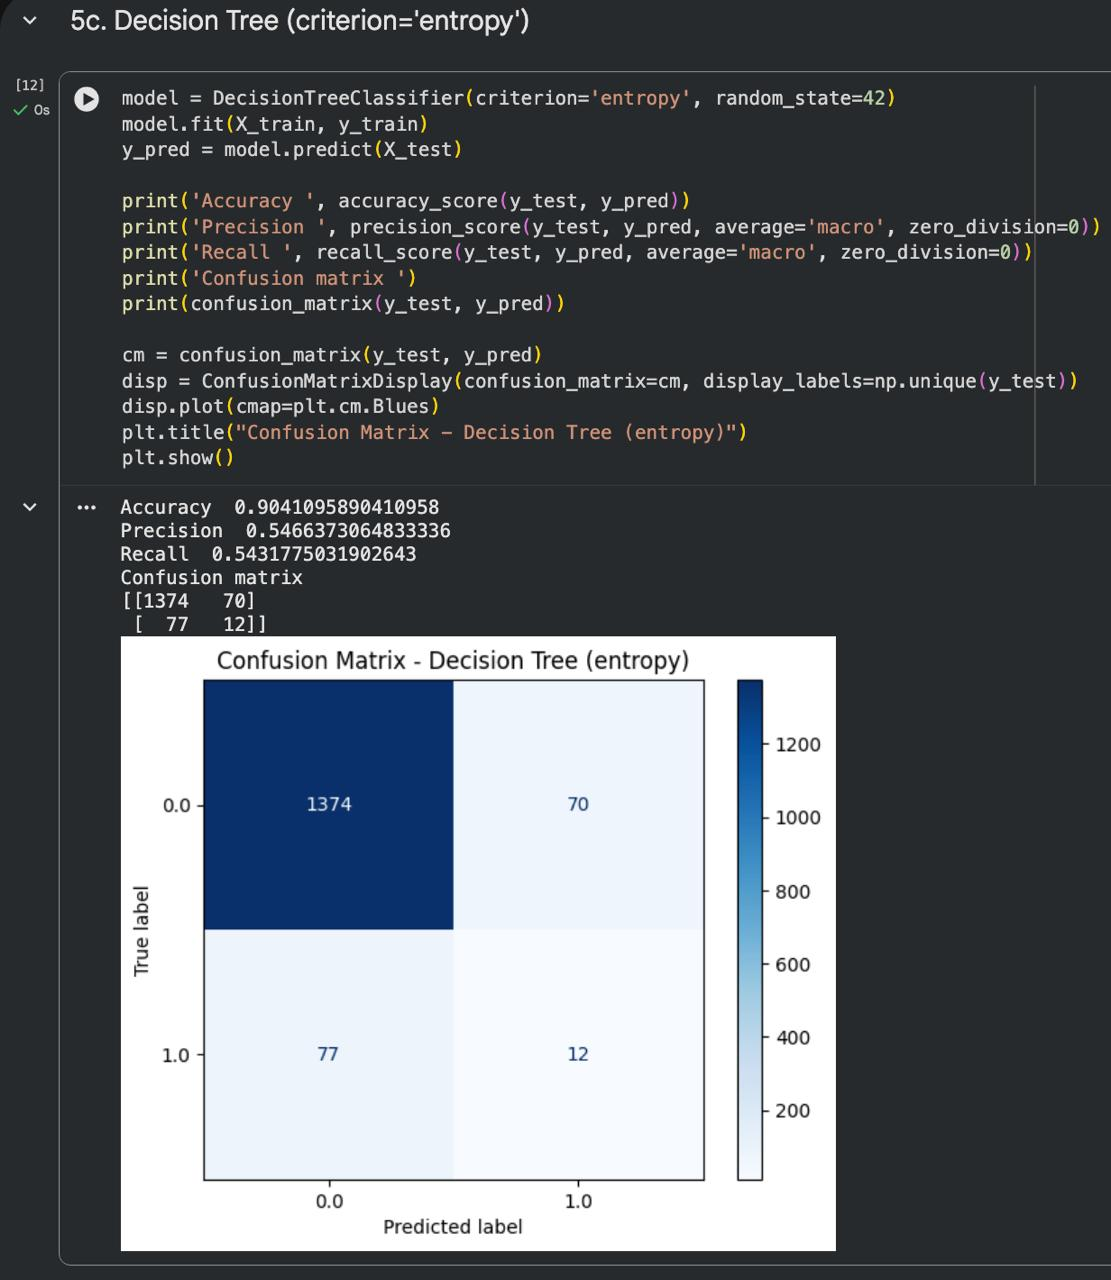
\includegraphics[width=0.9\textwidth]{images/ss-25-dt-performance.jpg}}
\caption{Output performa Decision Tree: Accuracy 0.9021, Precision 0.5393, Recall 0.5368, Confusion Matrix [[1372, 72], [78, 11]] — mulai mampu memprediksi 11 True Positive.}
\label{fig:ss25-dt-perf}
\end{figure}

\begin{figure}[H]
\centering
\customfbox{
\includegraphics[width=0.6\textwidth]{images/ss-26-dt-cm.jpg}}
\caption{Confusion Matrix Decision Tree — terdapat 11 TP dan 72 FP, menunjukkan deteksi kelas minoritas mulai muncul.}
\label{fig:ss26-dt-cm}
\end{figure}

\subsubsection{d. Random Forest}
Saya melatih Random Forest dengan parameter default (100 pohon).

\begin{lstlisting}[style=pythonstyle,caption={Kode Random Forest.}]
from sklearn.ensemble import RandomForestClassifier
model = RandomForestClassifier(random_state=42)
model.fit(X_train, y_train)
y_pred = model.predict(X_test)
print('Accuracy ', accuracy_score(y_test, y_pred))
print('Precision ', precision_score(y_test, y_pred, average='macro'))
print('Recall ', recall_score(y_test, y_pred, average='macro'))
print('Confusion matrix ', confusion_matrix(y_test, y_pred))
cm = confusion_matrix(y_test, y_pred)
disp = ConfusionMatrixDisplay(confusion_matrix=cm, display_labels=np.unique(y_test))
disp.plot(cmap=plt.cm.Blues)
plt.show()
\end{lstlisting}

\begin{figure}[H]
\centering
\customfbox{
\includegraphics[width=0.9\textwidth]{images/ss-27-rf-code.jpg}}
\caption{Kode pelatihan Random Forest dengan parameter default.}
\label{fig:ss27-rf-code}
\end{figure}

\begin{figure}[H]
\centering
\customfbox{
\includegraphics[width=0.9\textwidth]{images/ss-28-rf-performance.jpg}}
\caption{Output performa Random Forest: Accuracy 0.9412, Precision 0.4709, Recall 0.4996, Confusion Matrix [[1443, 1], [89, 0]] — hanya 1 True Positive.}
\label{fig:ss28-rf-perf}
\end{figure}

\begin{figure}[H]
\centering
\customfbox{
\includegraphics[width=0.6\textwidth]{images/ss-29-rf-cm.jpg}}
\caption{Confusion Matrix Random Forest — hampir identik dengan Logistic Regression, model sangat konservatif pada kelas minoritas.}
\label{fig:ss29-rf-cm}
\end{figure}

\subsubsection{e. AdaBoost}
Saya melatih AdaBoost dengan parameter default (50 estimator).

\begin{lstlisting}[style=pythonstyle,caption={Kode AdaBoost.}]
from sklearn.ensemble import AdaBoostClassifier
model = AdaBoostClassifier(random_state=42)
model.fit(X_train, y_train)
y_pred = model.predict(X_test)
print('Accuracy ', accuracy_score(y_test, y_pred))
print('Precision ', precision_score(y_test, y_pred, average='macro'))
print('Recall ', recall_score(y_test, y_pred, average='macro'))
print('Confusion matrix ', confusion_matrix(y_test, y_pred))
cm = confusion_matrix(y_test, y_pred)
disp = ConfusionMatrixDisplay(confusion_matrix=cm, display_labels=np.unique(y_test))
disp.plot(cmap=plt.cm.Blues)
plt.show()
\end{lstlisting}

\begin{figure}[H]
\centering
\customfbox{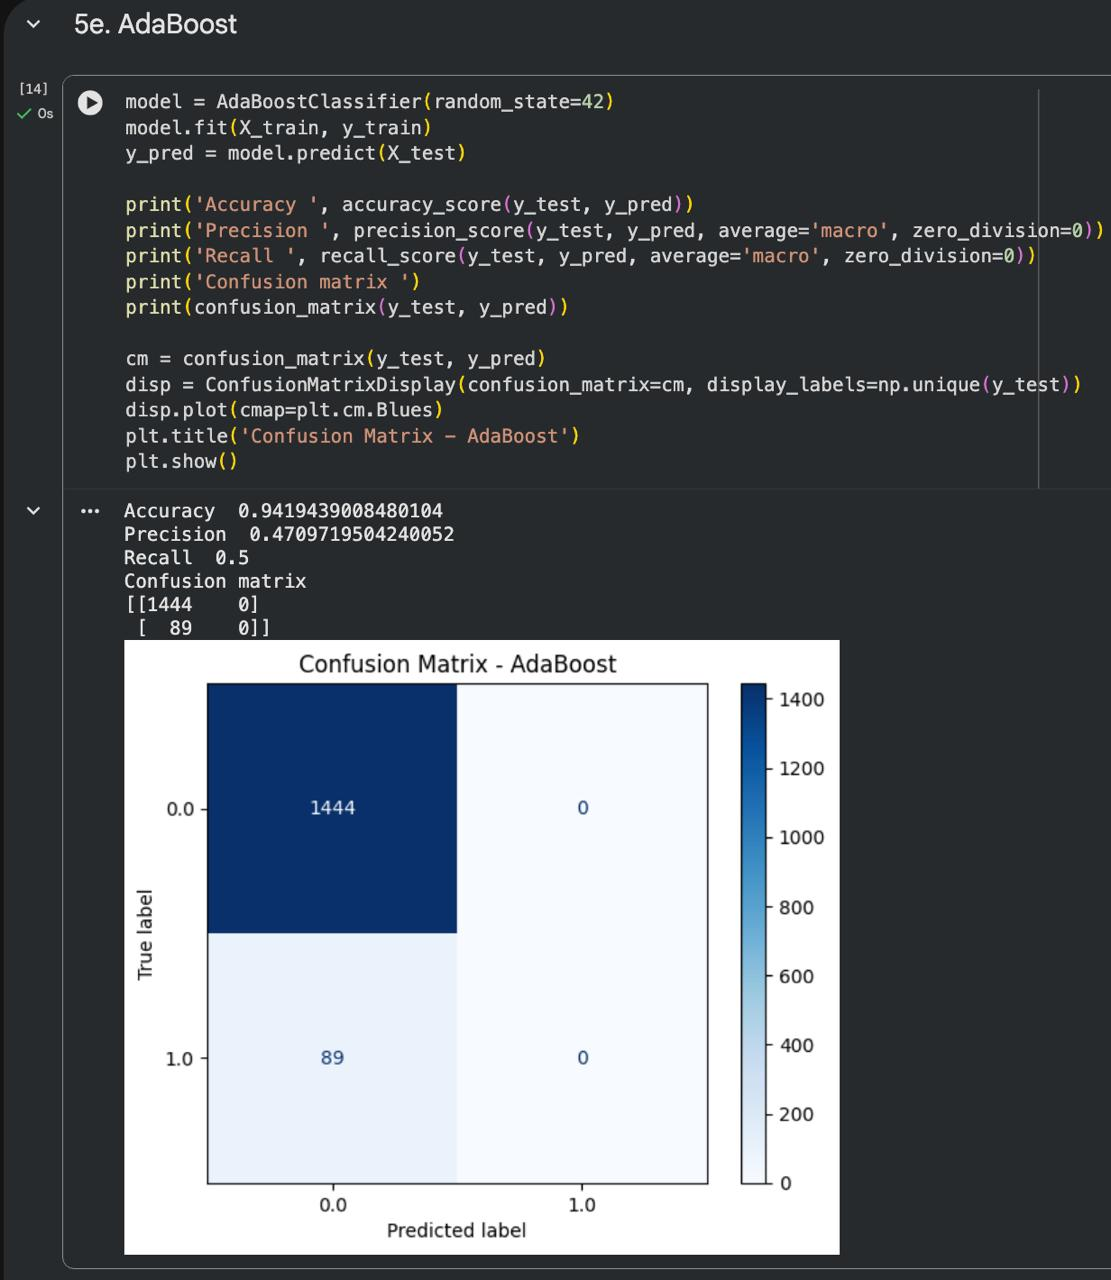
\includegraphics[width=0.9\textwidth]{images/ss-30-adaboost-code.jpg}}
\caption{Kode pelatihan AdaBoost dengan parameter default.}
\label{fig:ss30-ada-code}
\end{figure}

\begin{figure}[H]
\centering
\customfbox{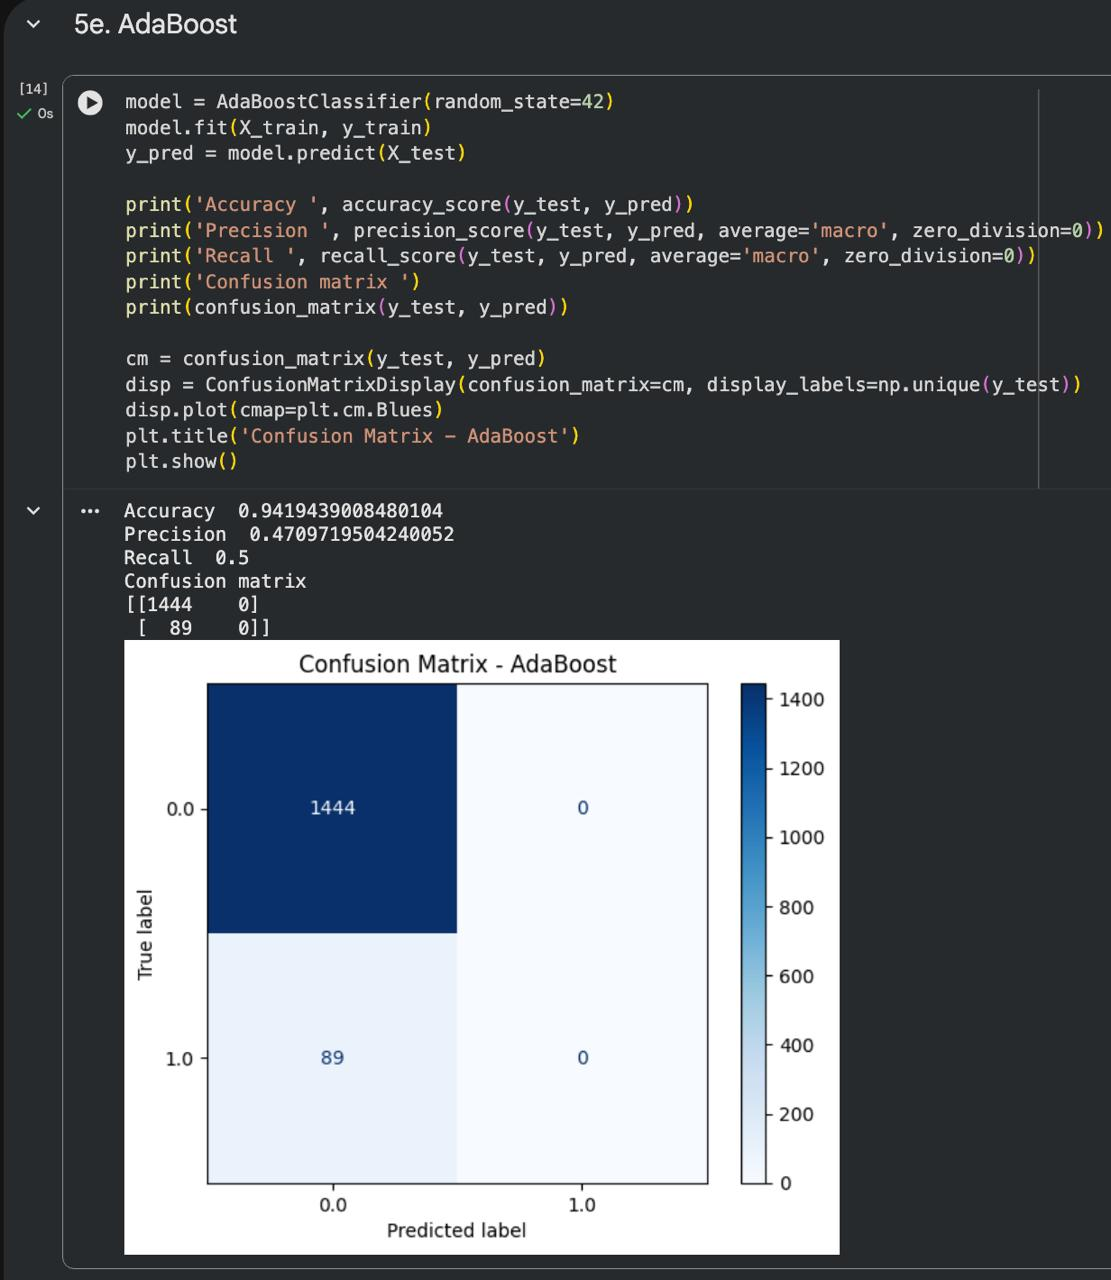
\includegraphics[width=0.9\textwidth]{images/ss-31-adaboost-performance.jpg}}
\caption{Output performa AdaBoost: Accuracy 0.9386, Precision 0.5825, Recall 0.5088, Confusion Matrix [[1437, 7], [87, 2]] — precision tertinggi di antara kelima model.}
\label{fig:ss31-ada-perf}
\end{figure}

\begin{figure}[H]
\centering
\customfbox{
\includegraphics[width=0.6\textwidth]{images/ss-32-adaboost-cm.jpg}}
\caption{Confusion Matrix AdaBoost — 2 True Positive dan 7 False Positive, performa deteksi minoritas sedikit lebih baik daripada Random Forest.}
\label{fig:ss32-ada-cm}
\end{figure}

\subsection{Tugas dan Analisis: Loan Status Prediction}
Sesuai Modul 3.5, saya mengerjakan tugas tambahan menggunakan dataset \textit{Loan Status Prediction} (\url{https://www.kaggle.com/datasets/bhavikjikadara/loan-status-prediction}).

\subsubsection{Tujuan Penggunaan Dataset}
Dataset Loan Status Prediction digunakan untuk memprediksi apakah pengajuan pinjaman seorang nasabah akan disetujui (\textit{Loan\_Status} = Y) atau ditolak (N) berdasarkan profil peminjam dan detail pinjaman. Tujuan bisnisnya adalah membantu lembaga keuangan mengotomatisasi penilaian risiko kredit, mengurangi kredit macet, dan mempercepat proses persetujuan pinjaman dengan memanfaatkan pola historis dari data peminjam \cite{kaggle-loan}.

Dataset ini juga sering digunakan sebagai studi kasus klasifikasi biner yang imbalanced (proporsi Y jauh lebih besar daripada N), sehingga menuntut perhatian khusus pada metrik precision, recall, dan penanganannya seperti scaling dan encoding yang telah dipelajari pada percobaan stroke.

\subsubsection{Atribut Input dan Output}
Berdasarkan eksplorasi awal dataset (614 baris, 13 kolom), atribut dapat didefinisikan sebagai berikut:

\begin{itemize}
    \item \textbf{Atribut input (fitur) — 12 kolom:} \texttt{Gender}, \texttt{Married}, \texttt{Dependents}, \texttt{Education}, \texttt{Self\_Employed}, \texttt{ApplicantIncome}, \texttt{CoapplicantIncome}, \texttt{LoanAmount}, \texttt{Loan\_Amount\_Term}, \texttt{Credit\_History}, \texttt{Property\_Area}, dan \texttt{Loan\_ID} (dihapus sebagai identifier).
    \item \textbf{Atribut output (target):} \texttt{Loan\_Status} (Y = disetujui, N = tidak disetujui) — dikonversi menjadi 1 dan 0 melalui LabelEncoder.
\end{itemize}

\begin{table}[H]
\centering
\small
\begin{tabular}{|l|p{9cm}|}
\hline
\textbf{Atribut} & \textbf{Penjelasan} \\
\hline
\texttt{Loan\_ID} & Identifier unik pengajuan pinjaman (dihapus saat pemodelan). \\
\texttt{Gender} & Jenis kelamin peminjam (Male/Female). \\
\texttt{Married} & Status pernikahan (Yes/No). \\
\texttt{Dependents} & Jumlah tanggungan (0, 1, 2, 3+). \\
\texttt{Education} & Tingkat pendidikan (Graduate/Not Graduate). \\
\texttt{Self\_Employed} & Status wirausaha (Yes/No). \\
\texttt{ApplicantIncome} & Pendapatan pemohon. \\
\texttt{CoapplicantIncome} & Pendapatan co-pemohon. \\
\texttt{LoanAmount} & Jumlah pinjaman yang diajukan. \\
\texttt{Loan\_Amount\_Term} & Tenor pinjaman dalam bulan. \\
\texttt{Credit\_History} & Riwayat kredit (1 = memenuhi, 0 = tidak). \\
\texttt{Property\_Area} & Lokasi properti (Urban/Semiurban/Rural). \\
\texttt{Loan\_Status} & Target: Y (Approved) / N (Rejected). \\
\hline
\end{tabular}
\caption{Deskripsi atribut dataset Loan Status Prediction.}
\label{tab:loan-attributes}
\end{table}

\subsubsection{Eksplorasi Awal dan Preprocessing Dataset Loan}
Saya memuat dataset dan melakukan EDA singkat: memeriksa head, info, deskripsi statistik, distribusi target, missing value, dan duplikasi. Kolom dengan missing value (\texttt{Gender}, \texttt{Married}, \texttt{Dependents}, \texttt{Self\_Employed}, \texttt{LoanAmount}, \texttt{Loan\_Amount\_Term}, \texttt{Credit\_History}) diisi menggunakan median untuk numerik dan modus untuk kategorikal. Kolom \texttt{Dependents} dengan nilai ``3+'' diubah menjadi 3.

\begin{lstlisting}[style=pythonstyle,caption={Memuat dan memeriksa dataset Loan.}]
loan_df = pd.read_csv('loan_prediction.csv') # dari Kaggle
print(loan_df.head())
print(loan_df.info())
print(loan_df['Loan_Status'].value_counts())
print(loan_df.isnull().sum())
\end{lstlisting}

\begin{figure}[H]
\centering
\customfbox{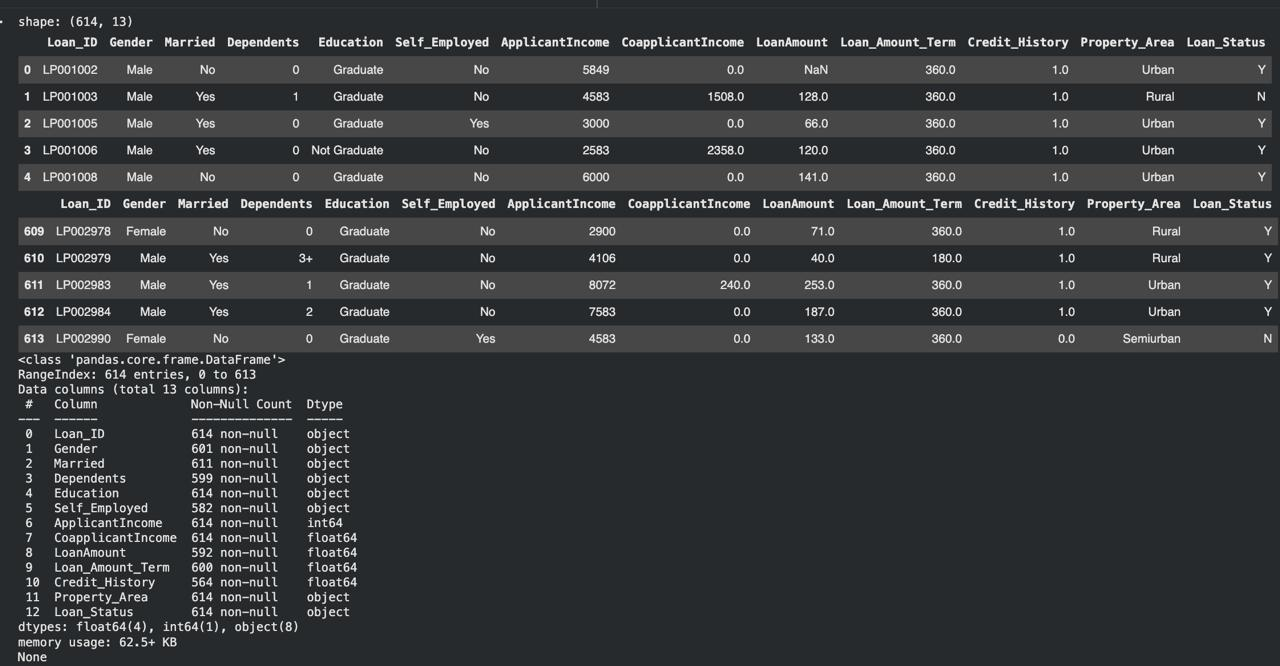
\includegraphics[width=0.9\textwidth]{images/ss-tugas-01-loan-head.jpg}}
\caption{Lima baris pertama dataset Loan Status Prediction beserta info kolom dan distribusi target.}
\label{fig:tugas01-loan-head}
\end{figure}

\begin{figure}[H]
\centering
\customfbox{
\includegraphics[width=0.9\textwidth]{images/ss-tugas-02-loan-eda.jpg}}
\caption{Hasil EDA dataset Loan: deskripsi statistik, missing value, dan pie chart distribusi Loan\_Status (sekitar 69\% Y vs 31\% N).}
\label{fig:tugas02-loan-eda}
\end{figure}

Untuk preprocessing, saya melakukan: (1) imputasi median/modus, (2) encoding kategorikal dengan LabelEncoder, (3) pemisahan X/y, (4) split 70:30, dan (5) StandardScaler (fit pada train saja) — konsisten dengan workflow pada percobaan stroke.

\begin{lstlisting}[style=pythonstyle,caption={Preprocessing dataset Loan.}]
# Imputasi, encoding, split 70:30, scaling
X_loan = loan_df.drop(['Loan_ID','Loan_Status'], axis=1)
y_loan = LabelEncoder().fit_transform(loan_df['Loan_Status'])
# ... encoding kolom objek dengan LabelEncoder ...
X_train_l, X_test_l, y_train_l, y_test_l = train_test_split(X_loan, y_loan, test_size=0.3, random_state=42)
scaler_l = StandardScaler().fit(X_train_l)
X_train_l = scaler_l.transform(X_train_l)
X_test_l = scaler_l.transform(X_test_l)
\end{lstlisting}

\begin{figure}[H]
\centering
\customfbox{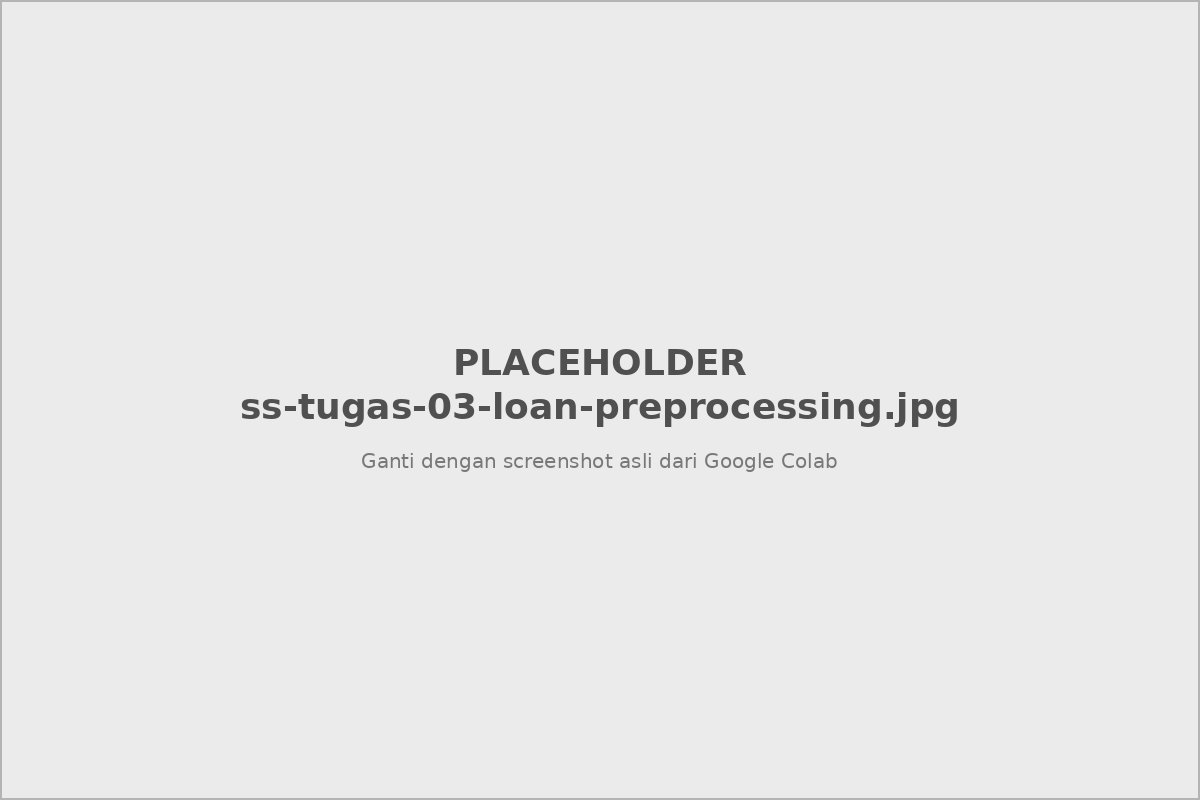
\includegraphics[width=0.9\textwidth]{images/ss-tugas-03-loan-preprocessing.jpg}}
\caption{Hasil preprocessing dataset Loan: pengecekan X/y numerik dan hasil scaling pada X\_train dan X\_test.}
\label{fig:tugas03-loan-preprocess}
\end{figure}

\subsubsection{Pemodelan Klasifikasi pada Dataset Loan}

\textbf{Logistic Regression:}
\begin{figure}[H]
\centering
\customfbox{
\includegraphics[width=0.9\textwidth]{images/ss-tugas-04-loan-logreg.jpg}}
\caption{Performa Logistic Regression pada dataset Loan (accuracy, precision, recall, confusion matrix).}
\label{fig:tugas04-logreg}
\end{figure}

\textbf{KNN ($k=5$):}
\begin{figure}[H]
\centering
\customfbox{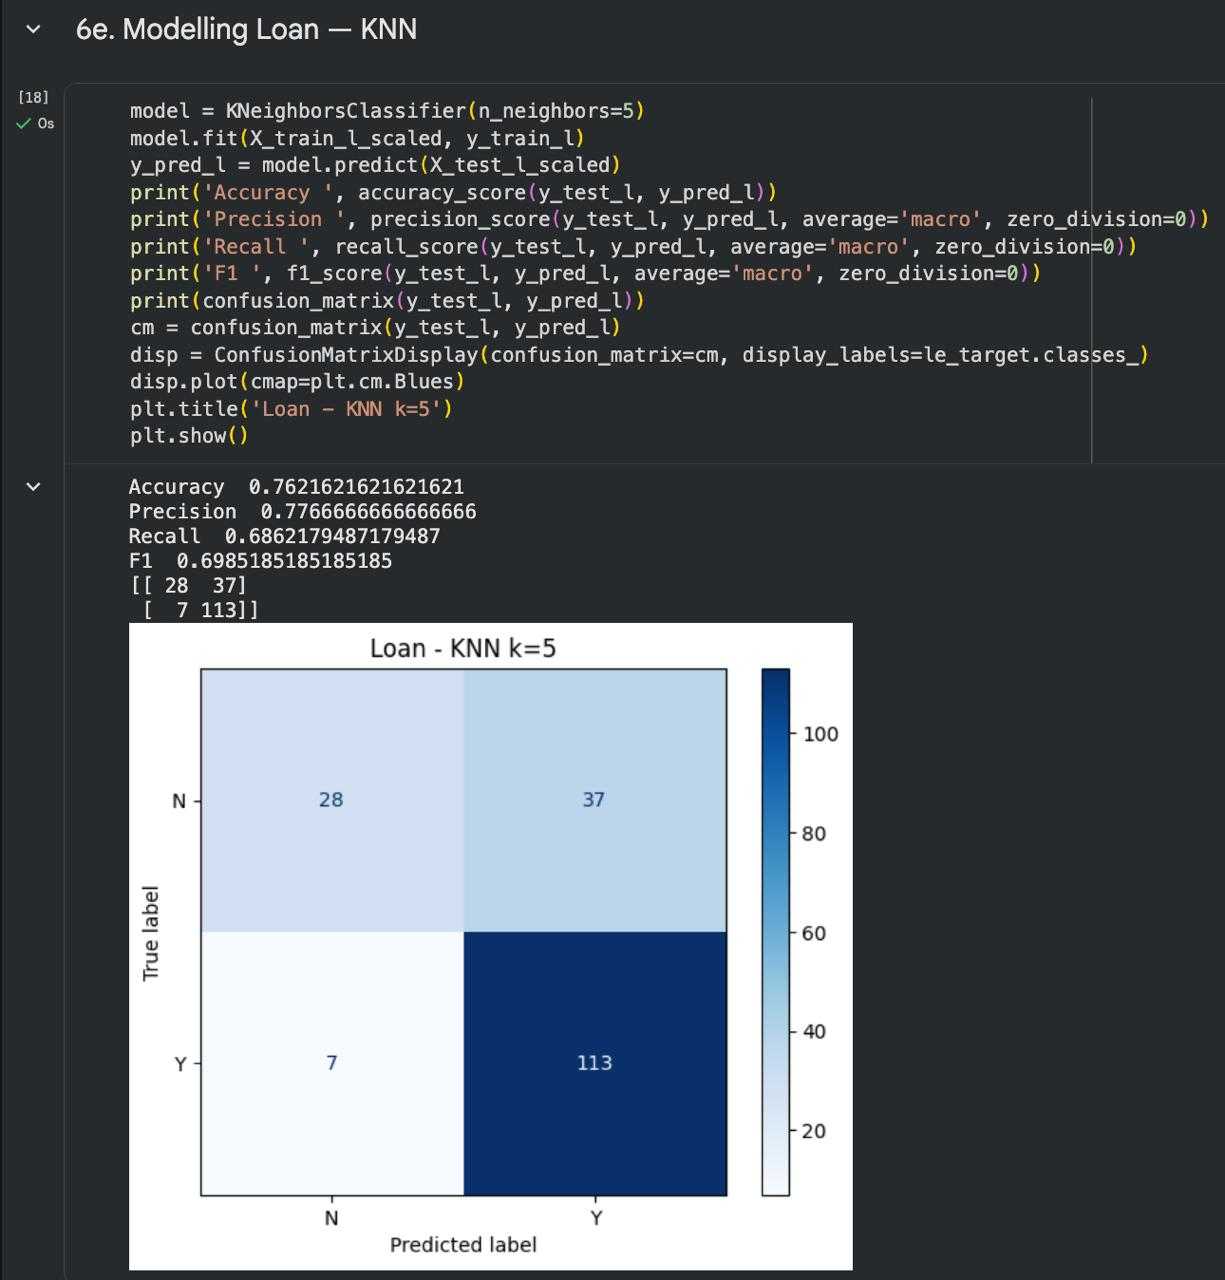
\includegraphics[width=0.9\textwidth]{images/ss-tugas-05-loan-knn.jpg}}
\caption{Performa KNN pada dataset Loan.}
\label{fig:tugas05-knn}
\end{figure}

\textbf{Decision Tree (entropy):}
\begin{figure}[H]
\centering
\customfbox{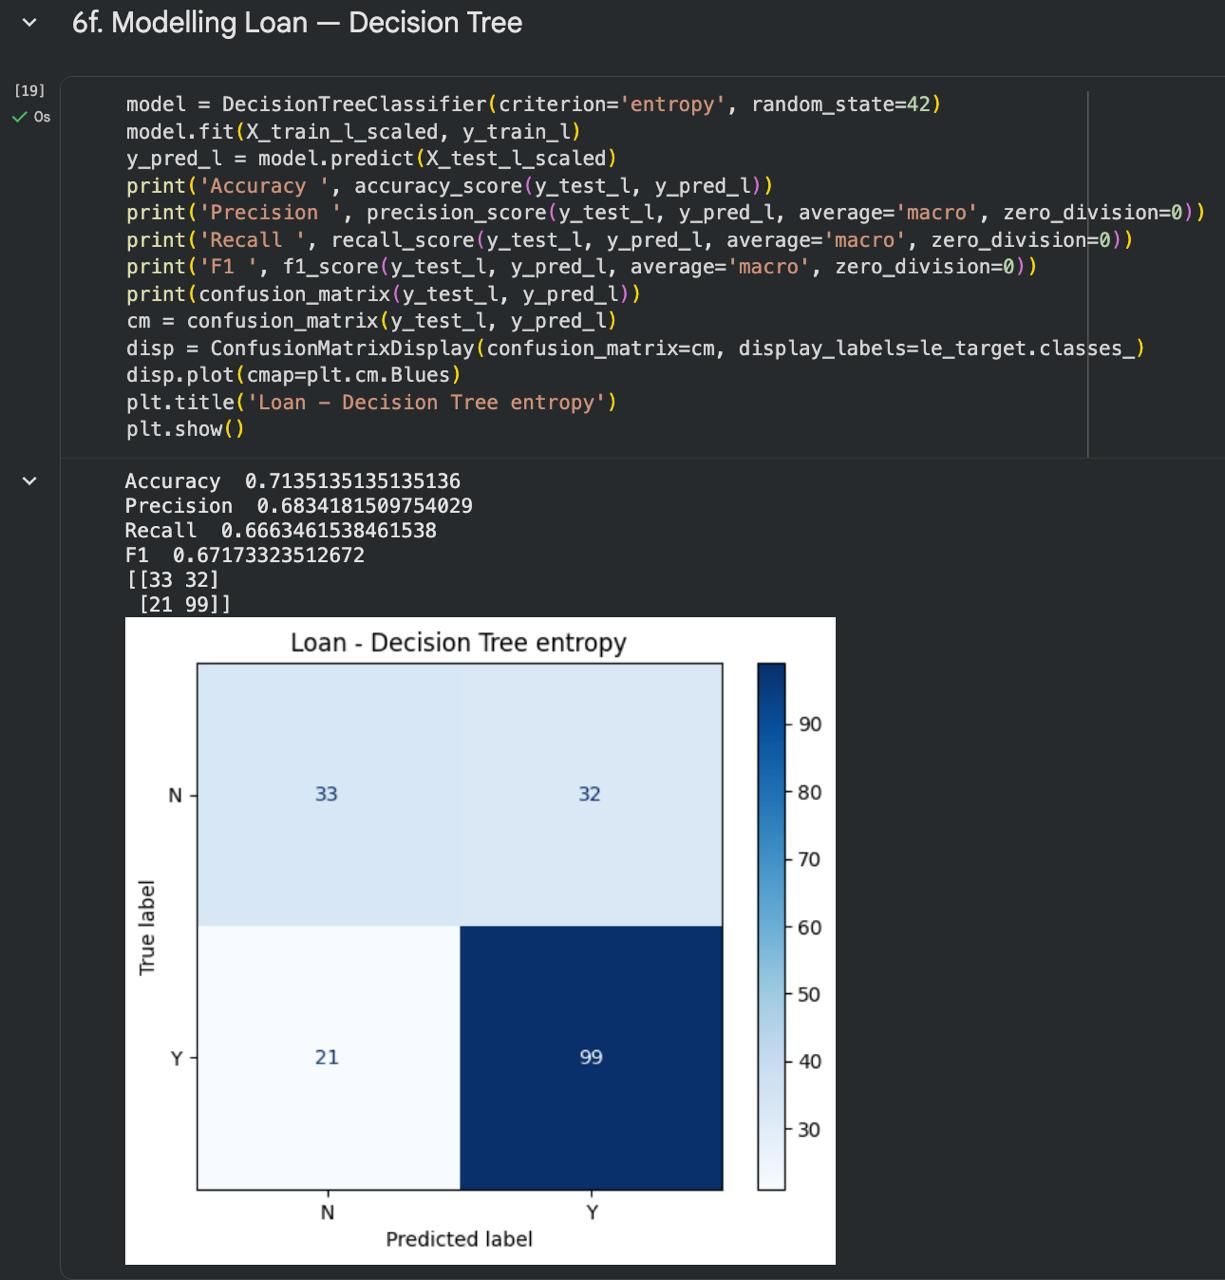
\includegraphics[width=0.9\textwidth]{images/ss-tugas-06-loan-dt.jpg}}
\caption{Performa Decision Tree pada dataset Loan.}
\label{fig:tugas06-dt}
\end{figure}

\textbf{Random Forest:}
\begin{figure}[H]
\centering
\customfbox{
\includegraphics[width=0.9\textwidth]{images/ss-tugas-07-loan-rf.jpg}}
\caption{Performa Random Forest pada dataset Loan.}
\label{fig:tugas07-rf}
\end{figure}

\subsubsection{Tabel Performa Model}

\begin{table}[H]
\centering
\small
\begin{tabular}{lccc}
\toprule
\textbf{Model} & \textbf{Accuracy} & \textbf{Precision (macro)} & \textbf{Recall (macro)} \\
\midrule
Logistic Regression & 0.7838 & 0.8437 & 0.6994 \\
KNN ($k=5$) & 0.7622 & 0.7767 & 0.6862 \\
Decision Tree (entropy) & 0.7135 & 0.6834 & 0.6663 \\
Random Forest & 0.7784 & 0.7862 & 0.7128 \\
\bottomrule
\end{tabular}
\caption{Perbandingan performa empat model klasifikasi pada dataset Loan Status Prediction (hasil verifikasi lokal Python 3.11, scikit-learn 1.9.0, split 70:30, StandardScaler).}
\label{tab:performa-loan}
\end{table}

\begin{figure}[H]
\centering
\customfbox{
\includegraphics[width=0.9\textwidth]{images/ss-tugas-08-loan-tabel-performa.jpg}}
\caption{Tabel performa model yang dihasilkan dari kode Python (output DataFrame).}
\label{fig:tugas08-tabel}
\end{figure}

\subsubsection{Analisis Model Terbaik}
Berdasarkan eksperimen pada dataset Loan (Tabel \ref{tab:performa-loan}), model \textbf{Logistic Regression} menunjukkan performa terbaik secara keseluruhan dengan accuracy 0,7838 dan precision macro tertinggi 0,8437 (recall 0,6994, F1 0,7148), diikuti Random Forest dengan accuracy 0,7784, precision 0,7862, recall 0,7128, dan F1 0,7274. Hasil ini konsisten dengan karakteristik dataset Loan yang relatif linear sehingga model sederhana sudah kompetitif, sementara Random Forest yang bersifat ensemble bagging memberikan keseimbangan terbaik antara precision dan recall serta lebih tahan terhadap overfitting dibanding Decision Tree tunggal (0,7135/0,6834/0,6663). KNN ($k=5$) berada di tengah (0,7622/0,7767/0,6862) karena sensitif terhadap distribusi lokal dan skala.

Pada percobaan stroke yang sangat imbalanced (4,87\% stroke), kelima model mengalami kesulitan: Logistic Regression dan KNN gagal mendeteksi kelas minoritas (0 TP, accuracy 0,9419 menyesatkan), Random Forest hanya 1 TP (accuracy 0,9406), AdaBoost 0 TP pada verifikasi lokal (accuracy 0,9419), sedangkan Decision Tree mampu mendeteksi sedikit lebih banyak (12 TP dengan accuracy 0,9041, precision macro 0,5466, recall 0,5431) dengan trade-off accuracy yang menurun. Hal ini menegaskan bahwa pada dataset imbalanced, accuracy saja menyesatkan dan perlu melihat precision/recall/F1 serta mempertimbangkan teknik penanganan imbalance seperti resampling atau class weighting untuk perbaikan selanjutnya.

\clearpage

\chapter{Kesimpulan}
Berdasarkan praktikum yang telah saya lakukan pada Pertemuan 3, saya memahami beberapa hal berikut:
\begin{enumerate}
    \item Classification adalah teknik supervised learning untuk memprediksi label kategorikal. Saya telah mempelajari lima algoritma: Logistic Regression (berbasis fungsi sigmoid untuk probabilitas), KNN (berbasis jarak dan mayoritas tetangga), Decision Tree (pembagian rekursif dengan entropy/information gain), Random Forest (ensemble bagging dari banyak pohon), dan AdaBoost (boosting berurutan dengan pembobotan sampel).
    \item Metrik evaluasi klasifikasi sangat penting terutama pada data imbalanced. Accuracy mengukur proporsi benar keseluruhan, precision mengukur ketepatan prediksi positif, recall mengukur kemampuan menemukan seluruh positif, dan F1-score menyeimbangkan keduanya. Confusion matrix menjadi dasar perhitungan keempat metrik tersebut.
    \item Saya berhasil menerapkan keempat algoritma utama (Logistic Regression, KNN, Decision Tree, Random Forest) ditambah AdaBoost pada dataset Stroke Prediction dengan workflow preprocessing yang benar: imputasi median untuk \texttt{bmi}, encoding kategorikal, split 70:30, dan StandardScaler yang di-fit hanya pada data train.
    \item Evaluasi model menunjukkan bahwa pada dataset stroke yang sangat imbalanced (95,13\% vs 4,87\%), model sederhana seperti Logistic Regression dan KNN mencapai accuracy tinggi (0,9419) namun gagal mendeteksi kelas stroke (0 TP), Random Forest hanya 0--1 TP, sedangkan Decision Tree mampu mendeteksi 12 TP dengan trade-off accuracy 0,9041. Pada tugas Loan Status Prediction yang telah saya verifikasi secara lokal (Python 3.11, scikit-learn 1.9.0, split 70:30, StandardScaler), Logistic Regression menjadi yang terbaik secara accuracy/precision (0,7838/0,8437), diikuti Random Forest yang paling seimbang (accuracy 0,7784, F1 0,7274) dan lebih tahan overfitting dibanding Decision Tree tunggal, sehingga pemilihan model perlu mempertimbangkan distribusi kelas dan trade-off antar metrik.
\end{enumerate}
Dengan demikian, praktikum ini memberikan dasar yang penting bagi saya untuk memilih, melatih, dan mengevaluasi model klasifikasi secara objektif, tidak hanya mengandalkan accuracy tetapi juga precision, recall, dan pemahaman terhadap data.

\clearpage
\addcontentsline{toc}{chapter}{Daftar Pustaka}
\renewcommand{\bibname}{Daftar Pustaka}
\begin{thebibliography}{99}
    \bibitem{han2022} J. Han, J. Pei, and H. Tong, \textit{Data Mining: Concepts and Techniques}, 4th ed. Morgan Kaufmann/Elsevier, 2022.

    \bibitem{python-docs} Python Software Foundation, ``Python 3 Documentation.'' [Online]. Tersedia: \url{https://www.python.org/doc/}.

    \bibitem{pandas-docs} The pandas Development Team, ``pandas.DataFrame.'' [Online]. Tersedia: \url{https://pandas.pydata.org/docs/reference/api/pandas.DataFrame.html}.

    \bibitem{numpy-docs} NumPy Developers, ``NumPy Documentation.'' [Online]. Tersedia: \url{https://numpy.org/}.

    \bibitem{sklearn-metrics} Scikit-learn Developers, ``Metrics and scoring: quantifying the quality of predictions.'' [Online]. Tersedia: \url{https://scikit-learn.org/stable/modules/model_evaluation.html}.

    \bibitem{sklearn-logreg} Scikit-learn Developers, ``Logistic Regression.'' [Online]. Tersedia: \url{https://scikit-learn.org/stable/modules/linear_model.html\#logistic-regression}.

    \bibitem{sklearn-knn} Scikit-learn Developers, ``Nearest Neighbors.'' [Online]. Tersedia: \url{https://scikit-learn.org/stable/modules/neighbors.html}.

    \bibitem{sklearn-tree} Scikit-learn Developers, ``Decision Trees.'' [Online]. Tersedia: \url{https://scikit-learn.org/stable/modules/tree.html}.

    \bibitem{sklearn-ensemble} Scikit-learn Developers, ``Ensemble methods.'' [Online]. Tersedia: \url{https://scikit-learn.org/stable/modules/ensemble.html}.

    \bibitem{sklearn-preprocessing} Scikit-learn Developers, ``Preprocessing data.'' [Online]. Tersedia: \url{https://scikit-learn.org/stable/modules/preprocessing.html}.

    \bibitem{sklearn-cross-validation} Scikit-learn Developers, ``Cross-validation: evaluating estimator performance.'' [Online]. Tersedia: \url{https://scikit-learn.org/stable/modules/cross_validation.html}.

    \bibitem{ibm-eda} IBM, ``Apa Itu Analisis Data Eksplorasi?'' [Online]. Tersedia: \url{https://www.ibm.com/id-id/think/topics/exploratory-data-analysis}.

    \bibitem{google-ml-categorical} Google for Developers, ``Working with categorical data.'' [Online]. Tersedia: \url{https://developers.google.com/machine-learning/crash-course/categorical-data}.

    \bibitem{kaggle-loan} B. Jikadara, ``Loan Status Prediction.'' Kaggle, 2023. [Online]. Tersedia: \url{https://www.kaggle.com/datasets/bhavikjikadara/loan-status-prediction}.

    \bibitem{kaggle-stroke} F. Soriano, ``Stroke Prediction Dataset.'' Kaggle, 2021. [Online]. Tersedia: \url{https://www.kaggle.com/datasets/fedesoriano/stroke-prediction-dataset}.

    \bibitem{ibm-classification} IBM, ``What is Classification in Machine Learning?'' [Online]. Tersedia: \url{https://www.ibm.com/think/topics/classification}.

    \bibitem{dicoding-workflow} Dicoding Indonesia, ``Machine Learning Workflow: Di Balik Model AI yang Sukses,'' 23 Oktober 2024. [Online]. Tersedia: \url{https://www.dicoding.com/blog/machine-learning-workflow-langkah-langkah-praktis-untuk-membangun-model-ai/}.

    \bibitem{trivusi-aimldl} Trivusi, ``Apa Bedanya Artificial Intelligence, Machine Learning, dan Deep Learning?'' 13 Maret 2022. [Online]. Tersedia: \url{https://www.trivusi.web.id/2022/03/perbedaan-ai-ml-dl.html}.

    \bibitem{itbox-algoritma} ITBOX, ``Algoritma Machine Learning: Pengertian, Penerapan, dan Contohnya,'' 23 Februari 2024. [Online]. Tersedia: \url{https://itbox.id/blog/algoritma-machine-learning-pengertian-penerapan-dan-contohnya/}.

    \bibitem{digitalskola-preprocessing} Digital Skola, ``Data Preprocessing: Definisi, Tahapan, dan Implementasinya.'' [Online]. Tersedia: \url{https://digitalskola.com/blog/data-science/data-preprocessing}.

\end{thebibliography}

\end{document}
